\documentclass[svgnames]{beamer}

\usepackage{pri}

\graphicspath{{./}{figures/}{figures/09-web-extraction-figs/}} 

\AtBeginSection[]
{
  \begin{frame}<beamer>
    \frametitle{Outline}
    \tableofcontents[currentsection,hideothersubsections]
  \end{frame}
}


\definecolorseries{tagcolor}{hsb}{grad}{DarkBlue}{.987,-.234,0}
\resetcolorseries[12]{tagcolor}
\newcounter{curtagcolor}
\setcounter{curtagcolor}{0}

\newcommand{\xbtag}[1]{\textcolor{tagcolor!![\thecurtagcolor]}{$<$\texttt{#1}$>$}}
\newcommand{\xetag}[1]{\textcolor{tagcolor!![\thecurtagcolor]}{$<$\texttt{/#1}$>$}}

\newcommand{\xabtag}[2]{\textcolor{tagcolor!![\thecurtagcolor]}{$<$\texttt{#1 \textcolor{black}{#2}}$>$}}

\newcommand{\xtag}[2]{\xbtag{#1}#2\xetag{#1}}
\newcommand{\xctag}[2]{\xbtag{#1}\addtocounter{curtagcolor}{1}#2\addtocounter{curtagcolor}{-1}\xetag{#1}}
\newcommand{\xenv}[2]{%
  \xbtag{#1}\addtocounter{curtagcolor}{1}\+\\
  #2\addtocounter{curtagcolor}{-1}\-\\
  \xetag{#1}}

\newcommand{\xatag}[3]{\xabtag{#1}{#2}#3\xetag{#1}}
\newcommand{\xaenv}[3]{%
  \xabtag{#1}{#2}\addtocounter{curtagcolor}{1}\+\\
  #3\addtocounter{curtagcolor}{-1}\-\\
  \xetag{#1}}

\newcommand{\doctype}[2]{%
  \textcolor{tagcolor!![\thecurtagcolor]}{$<$\texttt{!DOCTYPE #1 [}}\addtocounter{curtagcolor}{1}\+\\
  #2\addtocounter{curtagcolor}{-1}\-\\
  \textcolor{tagcolor!![\thecurtagcolor]}{\texttt{]}$>$}}

\newcommand{\attlist}[2]{%
  \textcolor{tagcolor!![\thecurtagcolor]}{$<$\texttt{!ATTLIST #1}}\+\+\\
  #2\textcolor{tagcolor!![\thecurtagcolor]}{$>$}\-\-}

\newenvironment{xml}{
  \begin{minipage}{.6\textwidth}
    \begin{tabbing}
      ---\=---\=---\=---\=---\=---\=\kill}{   
    \end{tabbing}
  \end{minipage}
}


\subtitle{Web Data Extraction}


\begin{document}

\maketitle
\makeoutline

\section{Introduction}

\begin{frame} \frametitle{Introduction}
  
  \begin{itemize}
  \item A large amount of information on the Web is contained in regularly
    structured data objects
    \begin{itemize}
    \item often data records retrieved from databases
    \end{itemize}
  \item Such Web data records are important:
    \begin{itemize}
    \item lists of products and services;
    \item Applications: e.g., comparative shopping, meta-search, meta-query,
      etc.
    \end{itemize}
  \end{itemize}

\end{frame}

% ------------------------------------------------------------

\begin{frame} \frametitle{Web Data Pages}

  There are two types of data rich pages:
  \begin{itemize}
  \item List pages
    \begin{itemize}
    \item Each such page contains one or more lists of data records
    \item Each list in a specific region in the page
    \item Two types of data records: \emph{flat} and \emph{nested}
    \end{itemize}
  \item Detail pages
    \begin{itemize}
    \item Each such page focuses on a single object
    \item But can have a lot of related and unrelated information
    \end{itemize}
  \end{itemize}
  
\end{frame}

% ------------------------------------------------------------

\begin{frame} \frametitle{A List Page}

  \centering
  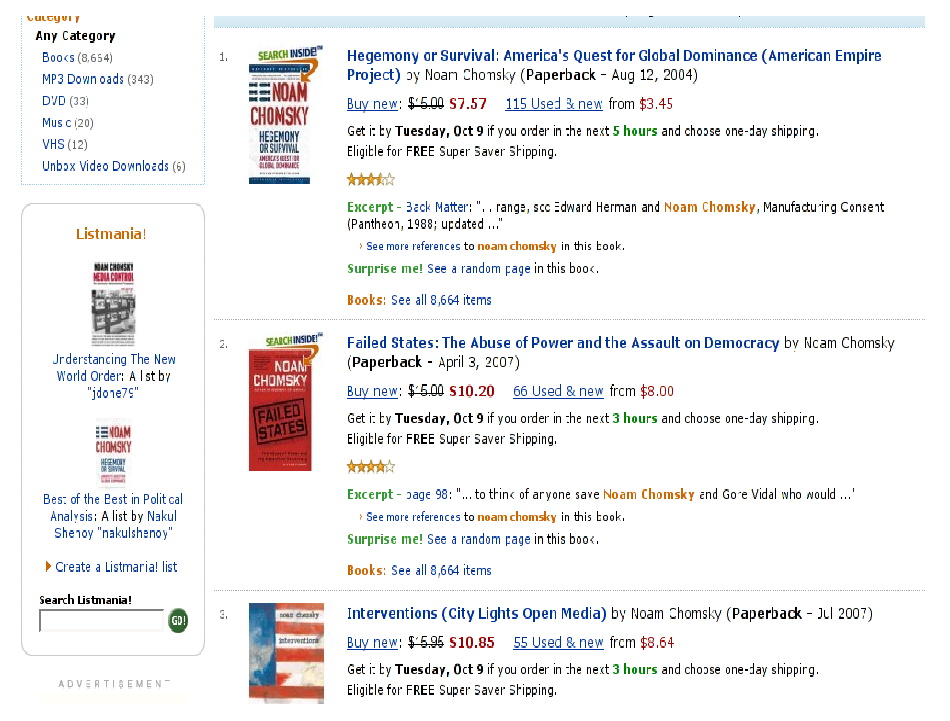
\includegraphics[width=\linewidth]{example1}
  
\end{frame}

% ------------------------------------------------------------

\begin{frame} \frametitle{A Detail Page}

  \centering
  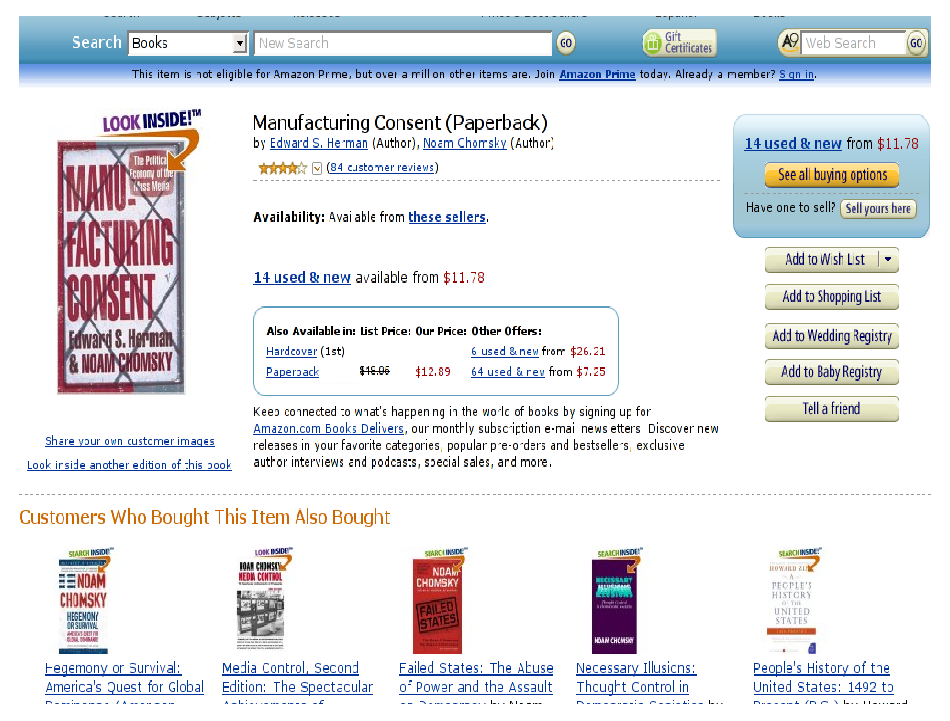
\includegraphics[width=\linewidth]{example2}
  
\end{frame}

% ------------------------------------------------------------

\begin{frame} \frametitle{Extraction Results}
  
  \centering
  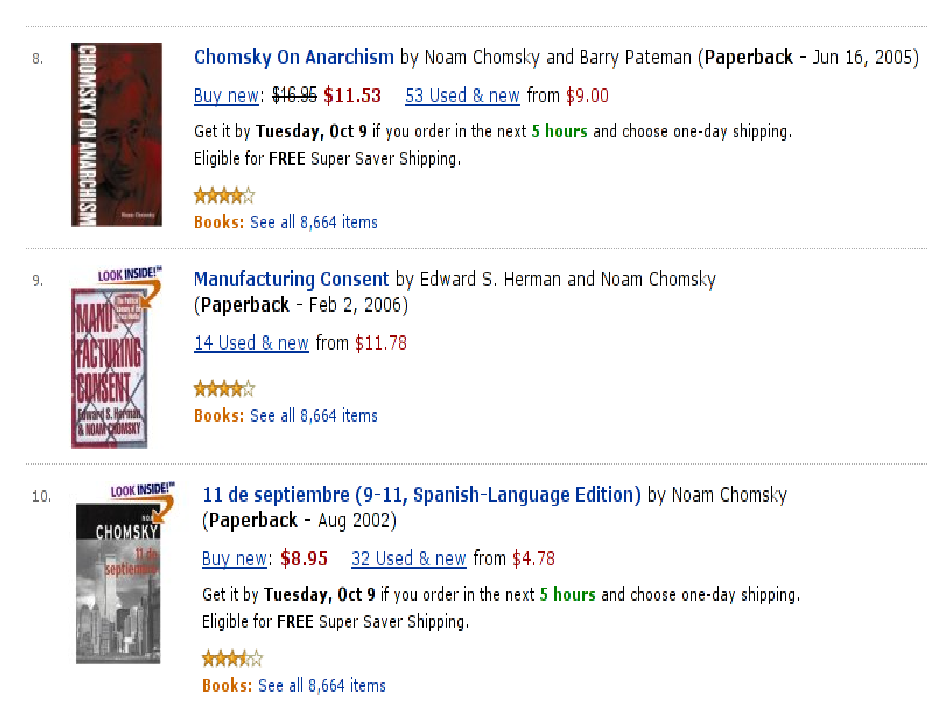
\includegraphics[width=.7\linewidth]{example3}\\
  \vfill
  \footnotesize
  \begin{tabular}{|l|l|c|c|}\hline
    Chomsky On Anarchism & Noam Chomsky, ... & \$11.53 & 4 \\\hline
    Manufacturing Consent & Edward S. Herman, ... & \$11.78 & 4 \\\hline
    11 de septiembre... & Noam Chomsky & \$8.95 & 3.5 \\\hline
    Imperial Grand Strategy... & Noam Chomsky & \$17.99 & 5 \\\hline
  \end{tabular}

\end{frame}

% ------------------------------------------------------------

\begin{frame}
    \frametitle{Extracting Web Data}

    \begin{itemize}
    \item To process this data implies extracting it from
        \emph{semi-structured} web pages and converting it to \emph{structured}
        information
    \item This is done by using \emph{wrappers}
    \end{itemize}

\end{frame}

\begin{frame} \frametitle{Wrappers}
  
  \begin{itemize}
  \item Wrappers are small applications or scripts capable of extracting
    information from semi-structured sources, such as HTML
  \item Wrappers can be built manually
    \begin{itemize}
    \item E.g., using \emph{regular expressions}, XPath, XQuery, ...
    \end{itemize}
  \item Or automatically
    \begin{itemize}
    \item Using machine learning techniques
    \end{itemize}
  \end{itemize}

\end{frame}

% ------------------------------------------------------------

\begin{frame} \frametitle{Using Regular Expressions}
  
  \begin{exampleblock}{Example:}
      \small\ttfamily
      R = <html>.*<hr><br>(.+?)<br>Title:~(.+?)<br>Author:~(.+?)
      \phantom{R = }<br>Price:~(.+?).*</body></html>
  \end{exampleblock}

\end{frame}

% ------------------------------------------------------------

\begin{frame} \frametitle{Using XPath or XQuery}

    \begin{exampleblock}{Example:}
        \centering
        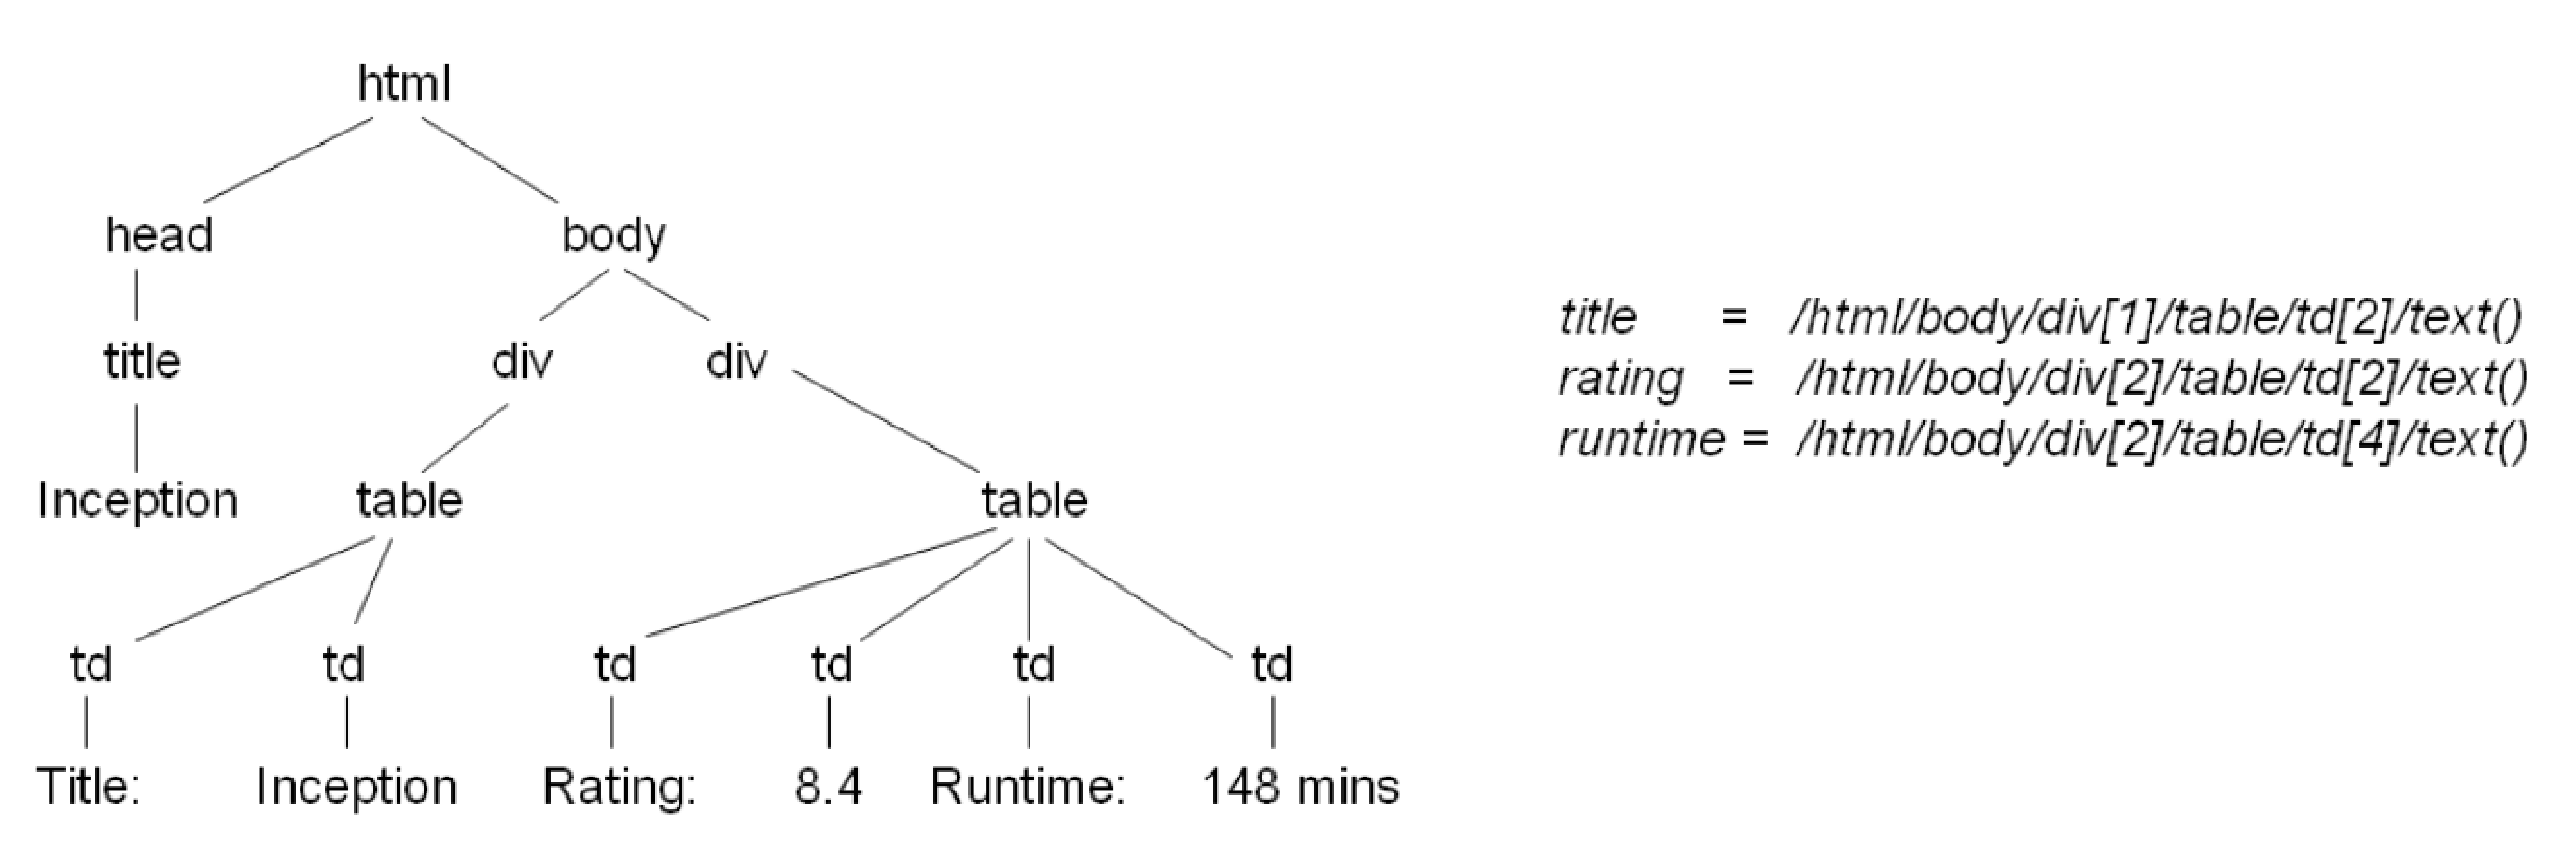
\includegraphics[width=\linewidth]{xpath_web_data}
    \end{exampleblock}
  
\end{frame}

% ------------------------------------------------------------

\begin{frame}
    \frametitle{Challenges of Building Wrappers}
    
    \begin{itemize}
    \item Learning the schema
        \begin{itemize}
        \item Similar to learning a grammar from examples (a well-known hard
            problem)
        \end{itemize}
    \item Learning the program
        \begin{itemize}
        \item Huge search space
        \end{itemize}
    \item Coping with exceptions
        \begin{itemize}
        \item Exceptions are commonplace on the Web
        \end{itemize}
    \end{itemize}

\end{frame}

\begin{frame} \frametitle{Limitations}
  
  \begin{itemize}
  \item Clearly, this mark-up encoding does not cover all cases in Web pages
    \begin{itemize}
    \item In fact, each group of a tuple type can be further divided
    \end{itemize}
  \item In an actual Web page the encoding may not be done by HTML tags alone
    \begin{itemize}
    \item Words and punctuation marks can be used
    \end{itemize}
  \end{itemize}

  \centering
  
\includegraphics[width=0.4\textwidth]{example4}

\end{frame}

% ------------------------------------------------------------

% \section{The Data Model and HTML Encoding}

% \begin{frame} \frametitle{The Data Model}

%   \begin{itemize}
%   \item Most Web data can be modeled as \emph{nested relations}
%     \begin{itemize}
%     \item typed objects allowing nested sets and tuples
%     \end{itemize}
%   \item An \emph{instance} of a type $T$ is simply an element of the domain of
%     $T$
%   \end{itemize}

%   \begin{definition}
%     \begin{itemize}
%     \item Let $B = \{B_1, B_2, \dotsc, B_k\}$ be a set of \emph{basic types}
%       \begin{itemize}
%       \item Each $B_i$ is atomic and of domain $dom(B_i)$
%       \end{itemize}
%     \item If $T_1, T_2, \dotsc, T_n$ are types, then $[T_1, T_2, \dotsc, T_n]$
%       is a \emph{tuple type} of domain $dom([T_1, T_2, \dotsc, T_n]) = \{[v_1,
%       v_2, \dotsc, v_n]|v_i \in dom(T_i)\}$
%     \item If $T$ is a tuple type, then $\{T\}$ is a \emph{set type} with domain
%       $dom(\{T\}) = 2^{dom(T)}$
%     \end{itemize}
%   \end{definition}

% \end{frame}

% % ------------------------------------------------------------

% \begin{frame} \frametitle{An Example Nested Tuple}
  
%   \begin{itemize}
%   \item Classic flat relations are of un-nested or flat set types
%   \item Nested relations are of arbitrary set types
%   \end{itemize}

%   \begin{exampleblock}{An example type}
%     \begin{tabbing}
%       \textbf{tuple} book (\=title:~~~~\=\textbf{string};\\
%                               \>author: \>\textbf{set} \=(name: \=\textbf{string});\\
%                               \>prices: \>\textbf{set} \>(\textbf{tuple} price (\=use: \=\textbf{string};\\
%                               \>       \>               \>                       \>price:\>~\textbf{number};))
%     \end{tabbing}
%   \end{exampleblock}

%   \begin{exampleblock}{An example tuple}
%     \vspace{-4.5ex}
%     \begin{multline*}
%       [\text{'Manufacturing Consent'}, \\
%       \{\text{'Edward S. Herman'},\text{'Noam Chomsky'}\}, \\
%       \{[\text{'used'}, 4.78],[\text{'new'}, 8.95]\}]
%     \end{multline*}
%   \end{exampleblock}

% \end{frame}

% % ------------------------------------------------------------

% \begin{frame} \frametitle{Type Trees}

%   \begin{definition}
%     \begin{itemize}
%     \item A basic type $B_i$ is a \emph{leaf}
%     \item A tuple type $[T_1, T_2, \dotsc, T_n]$ is a tree rooted at a
%       \emph{tuple node} with $n$ sub-trees, one for each $T_i$
%     \item A set type $\{T\}$ is a tree rooted at a \emph{set node} with one
%       sub-tree
%     \end{itemize}
%   \end{definition}

%   % We introduce a labeling of a type tree, which is defined recursively:
%   % \begin{itemize}
%   % \item If a set node is labeled $\Phi$, then its child is labeled $\Phi.0$
%   % \item If a tuple node is labeled $\Phi$, then its $n$ children are labeled
%   %   $\Phi.1, \dotsc, \Phi.n$
%   % \end{itemize}
  
% \end{frame}

% % ------------------------------------------------------------

% \begin{frame} \frametitle{An Example Type Tree}
  
%   \begin{exampleblock}{}
%     \centering
%     % \pstree[levelsep=8ex]{\TR{\textbf{tuple} \textit{(book)}}}{
%     %   \TR{\textbf{string} \textit{(title)}}
%     %   \pstree{\TR{\textbf{set} \textit{(author)}}}{
%     %     \TR{\textbf{string} \textit{(name)}}
%     %   }
%     %   \pstree{\TR{\textbf{set} \textit{(prices)}}}{
%     %     \pstree{\TR{\textbf{tuple} \textit{(price)}}}{
%     %       \TR{\textbf{string} \textit{(use)}}
%     %       \TR{\textbf{number} \textit{(price)}}
%     %     }
%     %   }
%     % }
%   \end{exampleblock}

%   \vfill
 
%   Note: attribute names are not part of the type tree.

% \end{frame}

% % ------------------------------------------------------------

% \begin{frame} \frametitle{Instance Trees}

%   \begin{definition}
%     \begin{itemize}
%     \item An instance (constant) of a basic type is a leaf
%     \item A tuple instance $[v_1, v_2, \dotsc, v_n]$ forms a tree rooted at a
%       tuple node with $n$ children or sub-trees representing attribute values
%       $v_1, v_2, \dotsc, v_n$
%     \item A set instance $\{e_1, e_2, \dotsc, e_n\}$ forms a set node with $n$
%       children or sub-trees representing the set elements $e_1, e_2, \dotsc,
%       e_n$
%     \end{itemize}
%   \end{definition}

%   \vfill

%   Note: A tuple instance is usually called a \emph{data record}
  
% \end{frame}

% % ------------------------------------------------------------

% \begin{frame} \frametitle{An Example Instance Tree}
  
%   \begin{exampleblock}{}
%     \centering
%     % \pstree[levelsep=8ex]{\TR{\textit{tuple}}}{
%     %   \TR{\shortstack{'Manufacturing\\Consent'}}
%     %   \pstree{\TR{\textit{set}}}{
%     %     \TR{\shortstack{'Edward\\S. Herman'}}
%     %     \TR{\shortstack{'Noam\\Chomsky'}}
%     %   }
%     %   \pstree{\TR{\textit{set}}}{
%     %     \pstree{\TR{\textit{tuple}}}{
%     %       \TR{'used'}
%     %       \TR{$4.78$}
%     %     }
%     %     \pstree{\TR{\textit{tuple}}}{
%     %       \TR{'new'}
%     %       \TR{$8.95$}
%     %     }
%     %   }
%     % }
%   \end{exampleblock}

% \end{frame}

% % ------------------------------------------------------------

% \begin{frame} \frametitle{HTML Encoding of Data}
  
%   \begin{itemize}
%   \item There are no designated tags for each type
%     \begin{itemize}
%     \item HTML was not designed as a data encoding language
%     \item Any HTML tag can be used for any type
%     \end{itemize}
%   \item For a tuple type, values (also called \emph{data items}) of different
%     attributes are usually encoded differently to distinguish them and to
%     highlight important items
%   \item A tuple may be partitioned into several groups or sub-tuples
%     \begin{itemize}
%     \item Each group covers a disjoint subset of attributes and may be encoded
%       differently
%     \end{itemize}
%   \end{itemize}

% \end{frame}

% % ------------------------------------------------------------

% \begin{frame} \frametitle{HTML Encoding and Type Trees}
  
%   \begin{definition}
%     For leaf node of a basic type $\Phi$, an instance $c$ is encoded with
%     \begin{displaymath}
%       enc(\Phi:c) = \text{OPEN-TAGS}~c~\text{CLOSE-TAGS}
%     \end{displaymath}
%     where \textit{OPEN-TAGS} is a sequence of open HTML tags and
%     \textit{CLOSE-TAGS} is a sequence of HTML close tags
%   \end{definition}

% \end{frame}

% % ------------------------------------------------------------

% \begin{frame} \frametitle{HTML Encoding and Type Trees (cont.)}
  
%   \begin{block}{}
%     A tuple node of type $[\Phi.1, \Phi.2, \dotsc, \Phi.n]$ is partitioned into
%     $h$ groups:
%     \begin{displaymath}
%       \langle\Phi.1, \dotsc, \Phi.e\rangle, \langle\Phi.(e+1), \dotsc,
%       \Phi.g\rangle, \dotsc, \langle\Phi.(k+1), \dotsc, \Phi.n\rangle
%     \end{displaymath}

%     An instance $[v_1, v_2, \dotsc, v_n]$ is encoded with:
%     \begin{multline*}
%       enc(\Phi:[v.1, v.2, \dotsc, v.n]) = \\
%       \text{OPEN-TAGS}_1~enc(v_1) \dotsb enc(v_e)~\text{CLOSE-TAGS}_1 \\
%       \text{OPEN-TAGS}_2~enc(v_{e+1}) \dotsb enc(v_g)~\text{CLOSE-TAGS}_2 \\
%       \dotsb \\
%       \text{OPEN-TAGS}_h~enc(v_{k+1}) \dotsb enc(v_n)~\text{CLOSE-TAGS}_h \\
%     \end{multline*}
%   \end{block}

% \end{frame}

% % ------------------------------------------------------------

% \begin{frame} \frametitle{HTML Encoding and Type Trees (cont.)}
  
%   \begin{block}{}
%     For a set node labeled $\Phi$, a non-empty set instance $\{e_1, e_2,
%     \dotsc, e_n\}$ is encoded with:
%     \begin{multline*}
%       enc(\Phi:\{e_1, e_2, \dotsc, e_n\}) = \\
%       \text{OPEN-TAGS}~enc(e_1), enc(e_2), \dotsc, enc(e_n)~\text{CLOSE-TAGS}
%     \end{multline*}
%   \end{block}

% \end{frame}

% % ------------------------------------------------------------

% \begin{frame} \frametitle{An Example}

%     \begin{columns}
%         \column{.5\linewidth}
%         \begin{exampleblock}{}
%             \small \centering
%             \begin{xml}
%                 \xenv{p}{
%                   \xtag{h3}{Manufacturing Consent}\\
%                   \xenv{ul}{
%                     \xtag{li}{Edward S. Herman}\\
%                     \xtag{li}{Noam Chomsky}
%                   }\\
%                   \xenv{ul}{ \xenv{li}{
%                       \xtag{strong}{used}\\
%                       \xtag{it}{4.78} } \xenv{li}{
%                       \xtag{strong}{new}\\
%                       \xtag{it}{8.95} } } }
%             \end{xml}
%         \end{exampleblock}
%         \column{.5\linewidth}
%         \small
%         $enc(string:\text{'Manuf...'}) =$ \xtag{h3}{Manuf...}\\[3ex]
%         $enc(tuple:[\text{'used'},4.78]) = $ \xtag{li}{$enc(string:\text{'used'})$$enc(num:4.78)$}\\[2ex]
%         $enc(string:\text{'used'}) =$ \xtag{strong}{used}\\[2ex]
%         $enc(num:4.78) =$ \xtag{it}{4.78}
%     \end{columns}

%     \centering
%     \emph{Goal:} discover $enc$

% \end{frame}

% % ------------------------------------------------------------

% \begin{frame} \frametitle{Limitations}
  
%   \begin{itemize}
%   \item Clearly, this mark-up encoding does not cover all cases in Web pages
%     \begin{itemize}
%     \item In fact, each group of a tuple type can be further divided
%     \end{itemize}
%   \item In an actual Web page the encoding may not be done by HTML tags alone
%     \begin{itemize}
%     \item Words and punctuation marks can be used
%     \end{itemize}
%   \end{itemize}

%   \centering
%   
\includegraphics[width=0.4\textwidth]{example4}

% \end{frame}

% ------------------------------------------------------------

\section{Wrapper Induction}

\begin{frame} \frametitle{Wrapper Induction}
  
  \begin{itemize}
  \item Wrappers are generated by using machine learning to generate extraction
    rules
    \begin{itemize}
    \item The user marks the target items in a few training pages
    \item The system learns extraction rules from these pages
    \item The rules are applied to extract items from other pages
    \end{itemize}
  \item There are many wrapper induction systems
    \begin{itemize}
    \item WIEN (Kushmerick et al, IJCAI-97)
    \item Softmealy (Hsu and Dung, 1998)
    \item BWI (Freitag and Kushmerick, AAAI-00)
    \item WL2 (Cohen et al. WWW-02)
    \item We will illustrate with \emph{Stalker} (Muslea et al. Agents-99)
    \end{itemize}
  \end{itemize}

\end{frame}

% ------------------------------------------------------------

% \begin{frame} \frametitle{Stalker: A Hierarchical Wrapper Induction System}

%   \begin{itemize}
%   \item Hierarchical wrapper learning
%     \begin{itemize}
%     \item Extraction is isolated at different levels of hierarchy
%     \item This is suitable for nested data records
%     \end{itemize}
%   \item Each item is extracted independently of others
%   \item The extraction is done using a tree structure called the \emph{EC~tree}
%     (embedded catalog tree)
%     \begin{itemize}
%     \item The EC tree is based on the type tree of the data
%     \end{itemize}
%   \item To extract each target item (a node), the wrapper needs a rule that
%     extracts the item from its parent
%   \end{itemize}
  
% \end{frame}

% ------------------------------------------------------------

\begin{frame} \frametitle{Extraction Rules}
  
  \begin{itemize}
  \item Each extraction is done using two rules
    \begin{itemize}
    \item a \emph{start rule} and an \emph{end rule}
    \end{itemize}
  \item The start rule identifies the beginning of the node and the end rule
    identifies the end of the node.
    \begin{itemize}
    \item This strategy is applicable to both leaf nodes (which represent data
      items) and list nodes
    \end{itemize}
  \item For a list node, \emph{list iteration rules} are needed to break the
    list into individual data records (tuple instances)
  \end{itemize}

\end{frame}

% ------------------------------------------------------------

% \begin{frame} \frametitle{Landmarks}
  
%   \begin{itemize}
%   \item The extraction rules are based on the idea of \emph{landmarks}
%     \begin{itemize}
%     \item A landmark is a sequence of consecutive tokens
%     \end{itemize}
%   \item Landmarks are used to locate the beginning and the end of a target
%     item
%   \item Rules use landmarks to extract the items
%   \end{itemize}

% \end{frame}

% ------------------------------------------------------------

\begin{frame} \frametitle{An Example}
  
  \begin{exampleblock}{}
    \centering \scriptsize
    \begin{xml}
      \xbtag{p}Seller Name:\xctag{b}{Good Books Inc.}\xbtag{br}\xbtag{br}\\
      \xctag{li}{321 Red Street, \xctag{i}{Mullen}, Phone
        0-\xctag{i}{485}-3463-1766} \\
      \xctag{li}{62 Blue Street, \xctag{i}{Finner}, Phone
        (621) 2176-2771} \\
      \xctag{li}{543 Yellow Street, \xctag{i}{Pitsher}, Phone
        0-\xctag{i}{788}-3452-4638} \\
      \xctag{li}{321 Orange Street, \xctag{i}{Kingston}, Phone:
        (333)-6755-7891}\xetag{p}
    \end{xml}
  \end{exampleblock}

  \begin{itemize}
  \item To extract the seller name, rule \textbf{R1} can identify the
    beginning:
    \begin{center}
      \textbf{R1:} \texttt{SkipTo(<b>)}
    \end{center}
  \item This rule means that the system should start from the beginning of the
    page and skip all the tokens until it sees the first \texttt{<b>} tag.
    \begin{itemize}
    \item \texttt{<b>} is a \emph{landmark}
    \end{itemize}
  \item Similarly, to identify the end of the seller name, we use:
    \begin{center}
      \textbf{R2:} \texttt{SkipTo(</b>)}
    \end{center}
  \end{itemize}

\end{frame}

% ------------------------------------------------------------

\begin{frame} \frametitle{An Example (cont.)}
  
  \begin{itemize}
  \item A rule may not be unique. For example, we can also use the following
    rules to identify the beginning of the name:
    \begin{center}
      \textbf{R3:} \texttt{SkiptTo(Name \_Punctuation\_ \_HtmlTag\_)}
    \end{center}
    or
    \begin{center}
      \textbf{R4:} \texttt{SkiptTo(Name) SkipTo(<b>)}
    \end{center}
  \item \textbf{R3} means that we skip everything untill the word "Name" followed
    by a punctuation symbol and then a HTML tag.
    \begin{itemize}
    \item In this case, ``\texttt{Name \_Punctuation\_ \_HtmlTag\_}'' together
      is a landmark
    \item \texttt{\_Punctuation\_} and \texttt{\_HtmlTag\_} are wildcards
    \end{itemize}

  \end{itemize}

\end{frame}

% ------------------------------------------------------------

\begin{frame} \frametitle{Learning Extraction Rules}
  
  Stalker uses \emph{sequential covering} to learn extraction rules for each
  target item
  \begin{itemize}
  \item In each iteration, it learns a perfect rule that covers as many
    positive examples as possible without covering any negative example
  \item Once a positive example is covered by a rule, it is removed
  \item The algorithm ends when all the positive examples are covered.
  \item The result is an ordered list of all learned rules
  \end{itemize}

\end{frame}

% ------------------------------------------------------------

\begin{frame} \frametitle{The Stalker Algorithm}
  
  \begin{block}{Algorithm LearnRules($examples$)}
    \begin{enumerate}
    \item $rule \leftarrow \emptyset$
    \item \textbf{while} $examples \neq \emptyset$ \textbf{do}
      \begin{enumerate}
      \item $disjunct \leftarrow LearnDisjunct(examples)$
      \item remove all items in $examples$ covered by $disjunct$
      \item add $disjunct$ to $rule$
      \end{enumerate}
    \item \textbf{return} $rule$
    \end{enumerate}
  \end{block}

\end{frame}

% ------------------------------------------------------------

\begin{frame} \frametitle{The Stalker Algorithm (cont.)}
  
  \begin{block}{Algorithm LearnDisjunct($examples$)}
    \begin{enumerate}
    \item $seed \leftarrow$ an example
    \item $candidates \leftarrow GetInitialCandidates(seed)$
    \item \textbf{while} $candidates \neq \emptyset$ \textbf{do}
      \begin{enumerate}
      \item $D \leftarrow BestDisjunct(candidates)$
      \item \textbf{if} $D$ is a perfect disjunct \textbf{then}
        \begin{enumerate}
        \item \textbf{return} $D$
        \end{enumerate}
      \item remove $D$ from $candidates$
      \item $candidates \leftarrow candidates \cup Refine(D,seed)$
      \end{enumerate}
    \item \textbf{return} $D$
    \end{enumerate}
  \end{block}

\end{frame}

% ------------------------------------------------------------

\begin{frame} \frametitle{The Stalker Algorithm (cont.)}
  
  \begin{block}{GetInitialCandidates($seed$)}
    Return tokens $t$ that immediately precede the example or wildcards that
    match $t$
  \end{block}

  \begin{block}{BestDisjunct($candidates$)}
    Return candidates that have
    \begin{itemize}
      \small
    \item more correct matches
    \item fewer false positives
    \item fewer wildcards
    \item longer landmarks
    \end{itemize}
  \end{block}

  \begin{block}{Refine($D,seed$)}
    Specialize $D$ by adding more terminals
  \end{block}

\end{frame}

% ------------------------------------------------------------

\begin{frame} \frametitle{An Example: Extracting Area Codes}
  
  \begin{exampleblock}{}
    \centering \scriptsize
    \begin{xml}
      E1:\xctag{li}{321 Red Street, \xctag{i}{Mullen}, Ph
        0-\xctag{i}{\colorbox{yellow}{485}}-3463-1766} \\
      E2:\xctag{li}{62 Blue Street, \xctag{i}{Finner}, Ph
        (\colorbox{yellow}{621}) 2176-2771} \\
      E3:\xctag{li}{543 Yellow Street, \xctag{i}{Pitsher}, Ph
        0-\xctag{i}{\colorbox{yellow}{788}}-3452-4638} \\
      E4:\xctag{li}{321 Orange Street, \xctag{i}{Kingston}, Ph:
        (\colorbox{yellow}{333})-6755-7891}\xetag{p}
    \end{xml}
  \end{exampleblock}

  \begin{itemize}
  \item Assume we start with \colorbox{yellow}{621}
  \item The following candidate disjuncts are generated: 
    \begin{itemize}
    \item[D1:] \texttt{SkipTo(\textit{(}) }
    \item[D2:] \texttt{SkipTo(\_Punctuation\_)}
    \end{itemize}
  \item D1 is selected by \texttt{BestDisjunct}
  \item D1 is a perfect disjunct
  \item The first iteration of \texttt{LearnRule()} ends
    \begin{itemize}
    \item E2 and E4 are removed
    \end{itemize}
  \end{itemize}

\end{frame}

% ------------------------------------------------------------

\begin{frame} \frametitle{An Example (cont.)}
  
  \begin{exampleblock}{}
    \centering \scriptsize
    \begin{xml}
      E1:\xctag{li}{321 Red Street, \xctag{i}{Mullen}, Ph
        0-\xctag{i}{\colorbox{yellow}{485}}-3463-1766} \\
      E3:\xctag{li}{543 Yellow Street, \xctag{i}{Pitsher}, Ph
        0-\xctag{i}{\colorbox{yellow}{788}}-3452-4638}
    \end{xml}
  \end{exampleblock}

  \begin{itemize}
  \item Two candidates are then generated:
    \begin{itemize}
    \item[D3:] \texttt{SkipTo(<i>)}
    \item[D4:] \texttt{SkipTo(\_HtmlTag\_)}
    \end{itemize}
  \item Both candidates match early in the uncovered examples, E1 and E3. Thus,
    they cannot uniquely locate the positive items
  \item Refinement is needed
  \end{itemize}

\end{frame}

% ------------------------------------------------------------

\begin{frame} \frametitle{Refinement}
  
  \begin{itemize}
  \item To specialize a disjunct by adding more \emph{terminals} to it
    \begin{itemize}
    \item A terminal means a token or one of its matching wildcards
    \end{itemize}
  \item We hope the refined version will be able to uniquely identify the
    positive items in some examples without matching any negative item in any
    example
  \item Two types of refinement:
    \begin{itemize}
    \item \emph{Landmark refinement}
    \item \emph{Topology refinement}
    \end{itemize}
  \end{itemize}

\end{frame}

% ------------------------------------------------------------

\begin{frame} \frametitle{Landmark Refinement}
  
  \emph{Landmark refinement}: increase the size of a landmark by concatenating
  a terminal

  \begin{exampleblock}{}
    \centering \scriptsize
    \begin{xml}
      E1:\xctag{li}{321 Red Street, \xctag{i}{Mullen}, Ph
        0-\xctag{i}{\colorbox{yellow}{485}}-3463-1766} \\
      E3:\xctag{li}{543 Yellow Street, \xctag{i}{Pitsher}, Ph
        0-\xctag{i}{\colorbox{yellow}{788}}-3452-4638}
    \end{xml}
  \end{exampleblock}

  \begin{itemize}
  \item[D5:] \texttt{SkipTo(-<i>)}
  \item[D6:] \texttt{SkipTo(\_Punctuation\_<i>)}
  \end{itemize}

\end{frame}

% ------------------------------------------------------------

\begin{frame} \frametitle{Topology Refinement}

  \emph{Topology refinement}: Increase the number of landmarks by adding
  1-terminal landmarks

  \begin{exampleblock}{}
    \centering \scriptsize
    \begin{xml}
      E1:\xctag{li}{321 Red Street, \xctag{i}{Mullen}, Ph
        0-\xctag{i}{\colorbox{yellow}{485}}-3463-1766} \\
      E3:\xctag{li}{543 Yellow Street, \xctag{i}{Pitsher}, Ph
        0-\xctag{i}{\colorbox{yellow}{788}}-3452-4638}
    \end{xml}
  \end{exampleblock}

  \begin{itemize}
    \small
  \item[D7] \texttt{SkipTo(321)SkipTo(<i>)}
  \item[D8] \texttt{SkipTo(Red)SkipTo(<i>)}
  \item[D9] \texttt{SkipTo(Street)SkipTo(<i>)}
  \item[D10] \texttt{SkipTo(,)SkipTo(<i>)}
  \item[D11] \texttt{SkipTo(<i>)SkipTo(<i>)}
  \item[...]
  \item[D19] \texttt{SkipTo(\_Numeric\_)SkipTo(<i>)}
  \item[D20] \texttt{SkipTo(\_Punctuation\_)SkipTo(<i>)}
  \end{itemize}

\end{frame}

% NOTE: at a certain point, you cannot refine more a given candidate, so you
% simply eliminate it. Thus teh set of candidates will eventually be empty.

% ------------------------------------------------------------

% NOTE: it is a true disjunction: there is no particular order in which the
% rules are executed.

\begin{frame} \frametitle{Final Results}
  
  \begin{exampleblock}{}
    \centering \scriptsize
    \begin{xml}
      E1:\xctag{li}{321 Red Street, \xctag{i}{Mullen}, Ph
        0-\xctag{i}{\colorbox{yellow}{485}}-3463-1766} \\
      E2:\xctag{li}{62 Blue Street, \xctag{i}{Finner}, Ph
        (\colorbox{yellow}{621}) 2176-2771} \\
      E3:\xctag{li}{543 Yellow Street, \xctag{i}{Pitsher}, Ph
        0-\xctag{i}{\colorbox{yellow}{788}}-3452-4638} \\
      E4:\xctag{li}{321 Orange Street, \xctag{i}{Kingston}, Ph:
        (\colorbox{yellow}{333})-6755-7891}\xetag{p}
    \end{xml}
  \end{exampleblock}

  \begin{itemize}
  \item Using \texttt{BestDisjunct}, D5 is selected as the final solution
    \begin{center}
      D5: \texttt{SkipTo(-<i>)}
    \end{center}
  \item Since all the examples are covered, \texttt{LearnRule()} returns the
    disjunctive (start) rule: either D1 or D5
    \begin{center}
      \textbf{R7:} \textbf{either} \texttt{SkipTo(\textit{(})} \textbf{or} \\
      \texttt{SkipTo(-<i>)}
    \end{center}
  \end{itemize}

\end{frame}

% ------------------------------------------------------------

% \begin{frame} \frametitle{Wrapper Maintenance}
  
%   \begin{itemize}
%   \item \emph{Wrapper verification}: if the site changes, does the wrapper know
%     the change?
%   \item \emph{Wrapper repair}: if the change is correctly detected, how to
%     automatically repair the wrapper?
%     \begin{itemize}
%     \item One way to deal with both problems is to learn the characteristic
%       patterns of the target items
%     \item These patterns are then used to monitor the extraction to check
%       whether the extracted items are correct
%     \end{itemize}
%   \item These tasks are extremely difficult
%     \begin{itemize}
%     \item often needs contextual and semantic information to detect changes and
%       to find the new locations of the target items
%     \end{itemize}
%   \item Wrapper maintenance is still an active research area
%   \end{itemize}

% \end{frame}

% ------------------------------------------------------------
% ------------------------------------------------------------
% ------------------------------------------------------------
% ------------------------------------------------------------

\section{Automatic Wrapper Generation}

\begin{frame} \frametitle{Problems of wrapper induction}
  
  Wrapper induction (supervised) has two main shortcomings:
  \begin{itemize}
  \item<2-> It is unsuitable for a large number of sites due to the manual labeling
    effort
  \item<3-> Wrapper maintenance is very costly.
    \begin{itemize}
    \item The Web is a dynamic environment.
    \item Sites change constantly.
    \item Since rules learnt by wrapper induction systems mainly use
      formatting tags, if a site changes its formatting templates, existing
      extraction rules for the site become invalid.
    \end{itemize}
  \end{itemize}

\end{frame}

% ------------------------------------------------------------

\begin{frame} \frametitle{Unsupervised learning}
  
    \begin{itemize}
    \item Due to these problems, automatic (or unsupervised) extraction has been
        studied
    \item Automatic extraction is possible because data records (tuple
        instances) in a Web site are usually encoded using a very small number
        of fixed templates
    \item It is possible to find these templates by \emph{mining repeated
          patterns}
    \end{itemize}
    
\end{frame}

% ------------------------------------------------------------

\begin{frame} \frametitle{The data extraction problem}
  
  \begin{itemize}
  \item We have an abstract model of structured data on the Web (i.e., nested
      relations), and a HTML mark-up encoding of the data model
  \item The general problem of data extraction is to \emph{recover the hidden
        schema} from the HTML mark-up encoded data
  \end{itemize}

\end{frame}

% ------------------------------------------------------------

\begin{frame}
    \frametitle{An Example}
    
    \begin{center}
        \includegraphics[width=.65\linewidth]{cap-schema}\\
        \texttt{schema = AB+C?D}
    \end{center}

    \begin{itemize}
    \item<2-> Note that, since we do not know the original schema, we do not know
        that \textit{A = title}, \textit{B = author}, etc.
    \end{itemize}

\end{frame}

% ------------------------------------------------------------

\section{Pattern Matching}

\begin{frame} \frametitle{Some useful algorithms}
  
  \begin{itemize}
  \item The key is to find the encoding template from a collection of
    encoded instances of the same type
  \item A natural way to do this is to detect repeated patterns from HTML
    encoding strings
  \item \emph{String edit distance} and \emph{tree edit distance} are obvious
    techniques for the task
  \end{itemize}

\end{frame}

% ------------------------------------------------------------

\begin{frame} \frametitle{String edit distance}
  
  \begin{itemize}
  \item String edit distance: the most widely used string comparison technique.
  \item The \emph{edit distance} of two strings, $s_1$ and $s_2$, is defined as
    the minimum number of point mutations required to change $s_1$ into $s_2$,
    where a point mutation is one of:
    \begin{enumerate}
    \item change a letter
    \item insert a letter
    \item delete a letter
    \end{enumerate}
  \end{itemize}

\end{frame}

% ------------------------------------------------------------

\begin{frame} \frametitle{A formal definition}
  
  \begin{block}{}
    \begin{itemize}
    \item For two string $s_1$ and $s_2$, the edit distance $d(s_1,s_2)$ is
      defined as:
      \begin{itemize}
      \item
        \begin{displaymath}
          d(\epsilon,\epsilon) = 0
        \end{displaymath}
      \item
        \begin{displaymath}
          d(s,\epsilon) = d(\epsilon,s) = |s|
        \end{displaymath}
      \item
        \begin{displaymath}
          \begin{split}
            d(s_1+c_1,s_2+c_2) = min(&d(s_1,s_2)+r(c_1,c_2), \\
            & d(s_1+c_1,s_2) + 1, \\
            & d(s_1,s_2+c_2) + 1
          \end{split}
        \end{displaymath}
      \end{itemize}
      where $r(c_1,c_2) = 0$ if $c_1=c_2$ and $r(c_1,c_2) = 1$ otherwise.
    \end{itemize}
  \end{block}

\end{frame}

% ------------------------------------------------------------

\begin{frame} \frametitle{Dynamic programming}
  
  \begin{itemize}
  \item We can use a matrix $m[0..|s_1|,0..|s_2|]$ to hold the edit distances
  \item The value in each cell is computed iteratively, from $m[0,0]$
  \item The last cell, $m[|s_1|,|s_2|]$ will hold the required value of edit
    distance
  \end{itemize}

  \begin{block}{}
    \begin{itemize}
    \item The matrix is defined as:
      \begin{itemize}
      \item $m[0,0] = 0$
      \item $m[i,0] = i$
      \item $m[0,j] = j$
      \item $m[i,j] = min(m[i-1,j-1)+r(s_1[i],s_2[j]), m[i-1,j]+1, m[i,j-1]+1)$
      \end{itemize}
    \end{itemize}
  \end{block}

\end{frame}

% ------------------------------------------------------------

\begin{frame} \frametitle{An example}
  
  \begin{itemize}
  \item To compute the edit distance between ``XGYXYXYX'' and ``XYXYXYTX''
  \end{itemize}

  \begin{center}
    \includegraphics[width=.5\linewidth]{dynamic}
  \end{center}

  \begin{itemize}
  \item The string alignment is
  \end{itemize}

  \begin{center}
    \ttfamily
    XGYXYXY-X \\
    X-YXYXYTX
  \end{center}

  %\small \uncover<2->{Question: How can this help in finding Web page
  %  templates?}

\end{frame}

% ------------------------------------------------------------

\begin{frame} \frametitle{Tree Edit Distance}
  
  \begin{itemize}
  \item Tree edit distance between two trees $A$ and $B$ (labeled ordered
    rooted trees) is the cost associated with the minimum set of operations
    needed to transform $A$ into $B$
  \item The set of operations used to define tree edit distance includes three
    operations:
    \begin{itemize}
    \item node removal
    \item node insertion
    \item node replacement
    \end{itemize}
  \item A cost is assigned to each of the operations
  \end{itemize}

\end{frame}

% ------------------------------------------------------------

\begin{frame} \frametitle{Definition}
  
  \begin{block}{}
    \begin{itemize}
    \item Let $X$ be a tree and $X[i]$ be the $i$-th node of $X$
    \item A mapping $M$ between a tree $A$ and a tree $B$ is a set of ordered
      pairs $(i,j)$, where $i$ is a node in tree $A$ and $j$ is a node in tree
      $B$, such that, for every $(i_1,j_1),(i_2,j_2) \in M$:
      \begin{enumerate}
      \item $i_1 = i_2$ iff $j_1 = j_2$
      \item $A[i_1]$ is on the left of $A[i_2]$ iff $B[j_1]$ is on the left of
        $B[j_2]$
      \item $A[i_1]$ is an ancestor of $A[i_2]$ iff $B[j_1]$ is an ancestor of
        $B[j_2]$
      \end{enumerate}
    \end{itemize}
  \end{block}

\end{frame}

% ------------------------------------------------------------

\begin{frame} \frametitle{An Example Mapping}

  \centering
  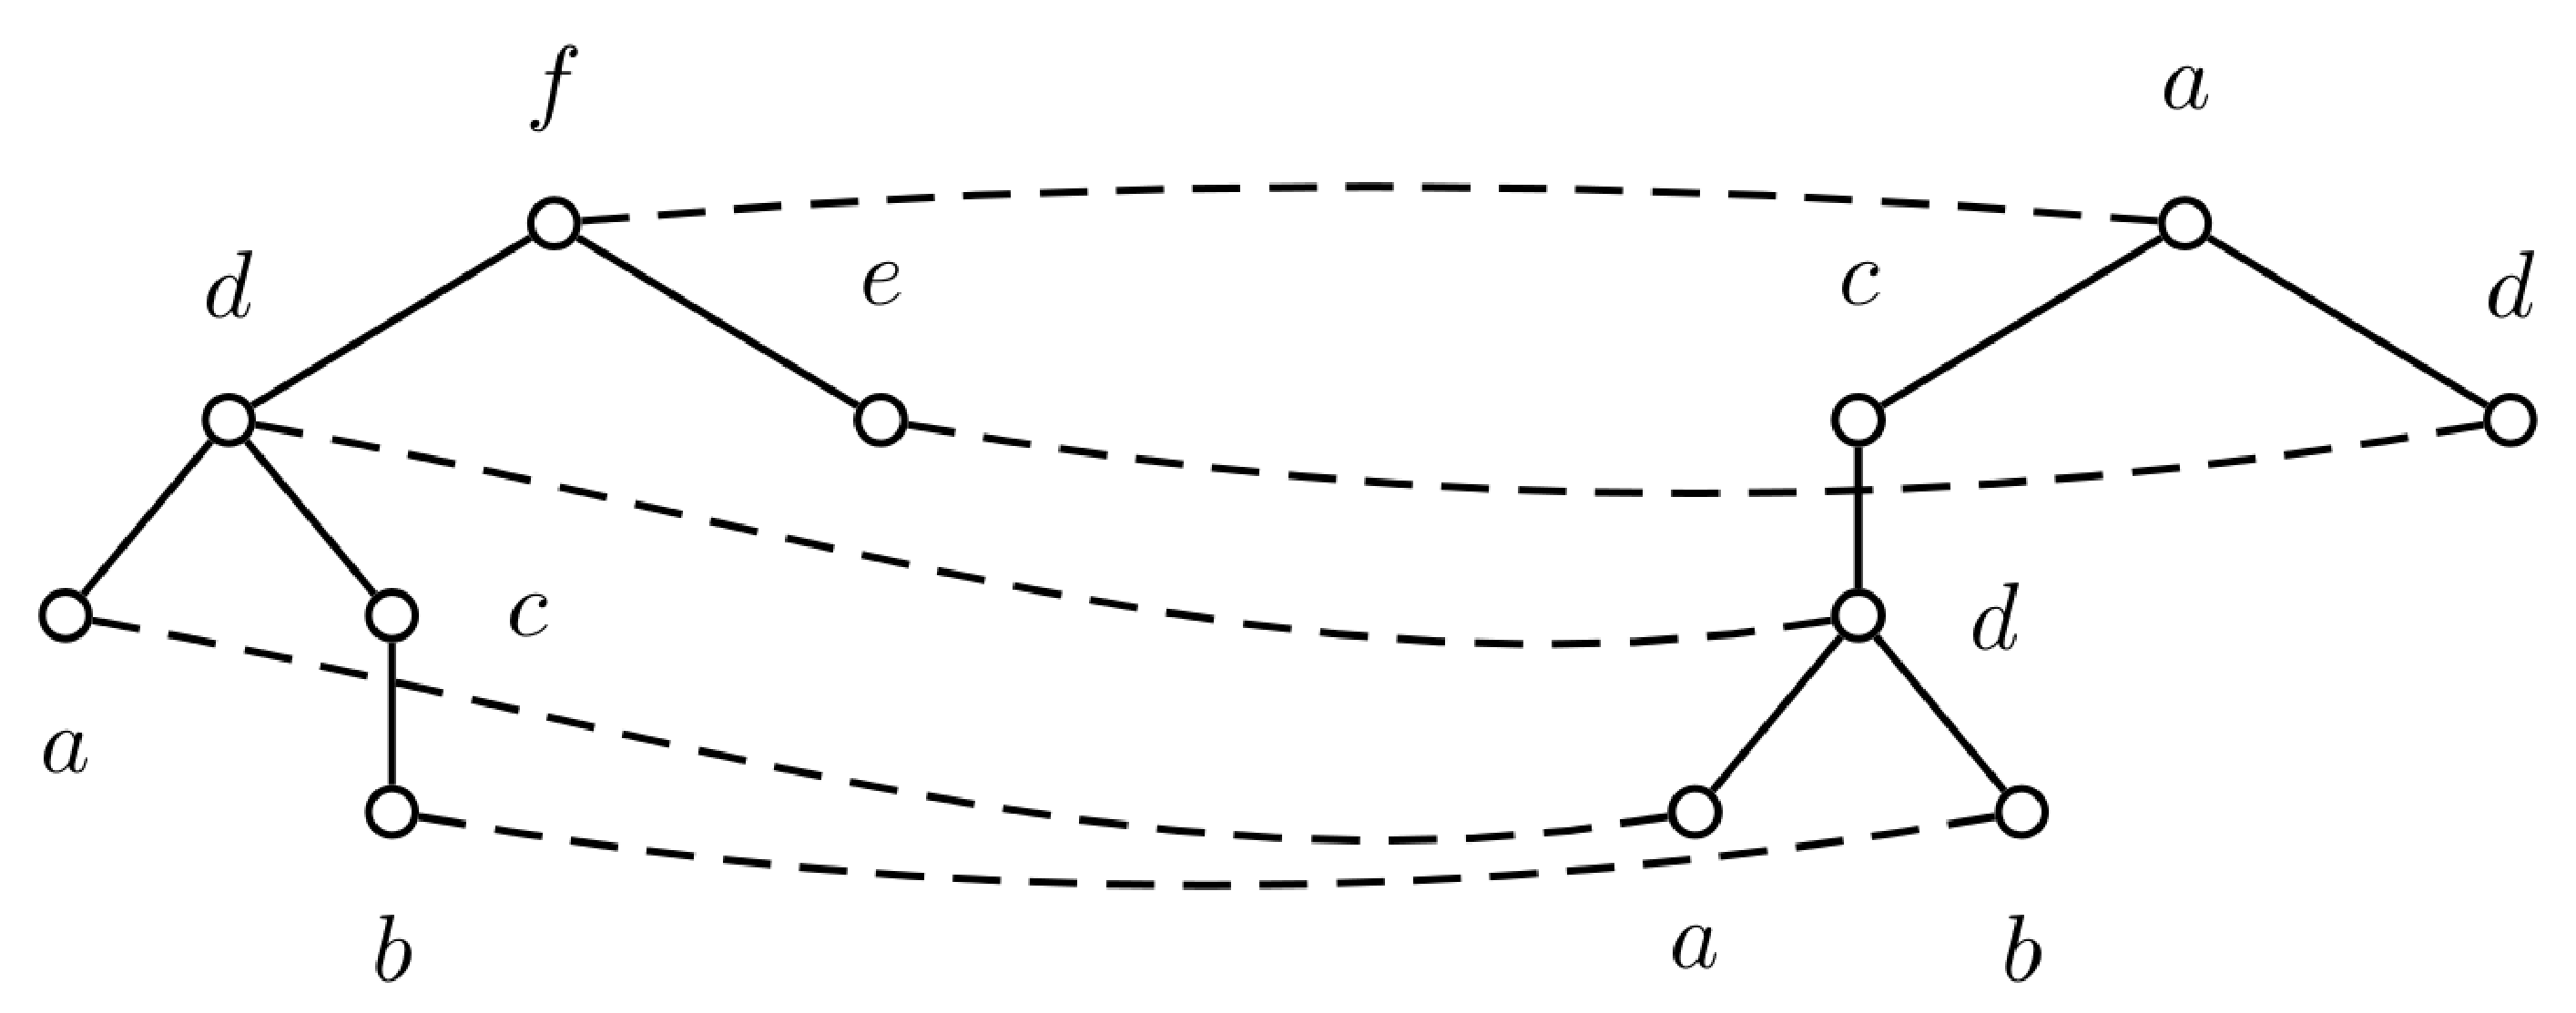
\includegraphics[width=\linewidth]{mapping}

\end{frame}

% ------------------------------------------------------------

\begin{frame} \frametitle{The tree matching problem}
  
    \begin{itemize}
    \item In the general setting:
        \begin{itemize}
        \item mapping can cross levels, e.g., node $d$ in tree A and node $d$
            in tree B.
        \item replacements are also allowed, e.g., node $f$ in A and node $a$
            in B
        \end{itemize}
    \item General matching/mapping algorithms are computationally complex
        \begin{itemize}
        \item In general $O(|A|^2|B|^2)$, although different solutions can have
            different complexities
        \end{itemize}
    \item In practice we can use more restrictive algorithms
    \item An example is \emph{Simple Tree Matching} (STM)
        \begin{itemize}
        \item Liu \& Zhai 2005
        \end{itemize}
    \end{itemize}

\end{frame}

% ------------------------------------------------------------


\begin{frame}
    \frametitle{Simple Tree Matching}

    \begin{itemize}
    \item STM is a top-down algorithm
    \item Instead of computing the edit distance of two trees, it evaluates
        their similarity by producing the maximum matching through dynamic
        programming
    \item Restrictions:
        \begin{itemize}
        \item Node labels must match
        \item Matching must occur at the same level
        \end{itemize}
    \item Complexity: $O(|A||B|)$
    \end{itemize}

\end{frame}

% ------------------------------------------------------------

\begin{frame} \frametitle{Simple Tree Matching algorithm}
  
  \centering
  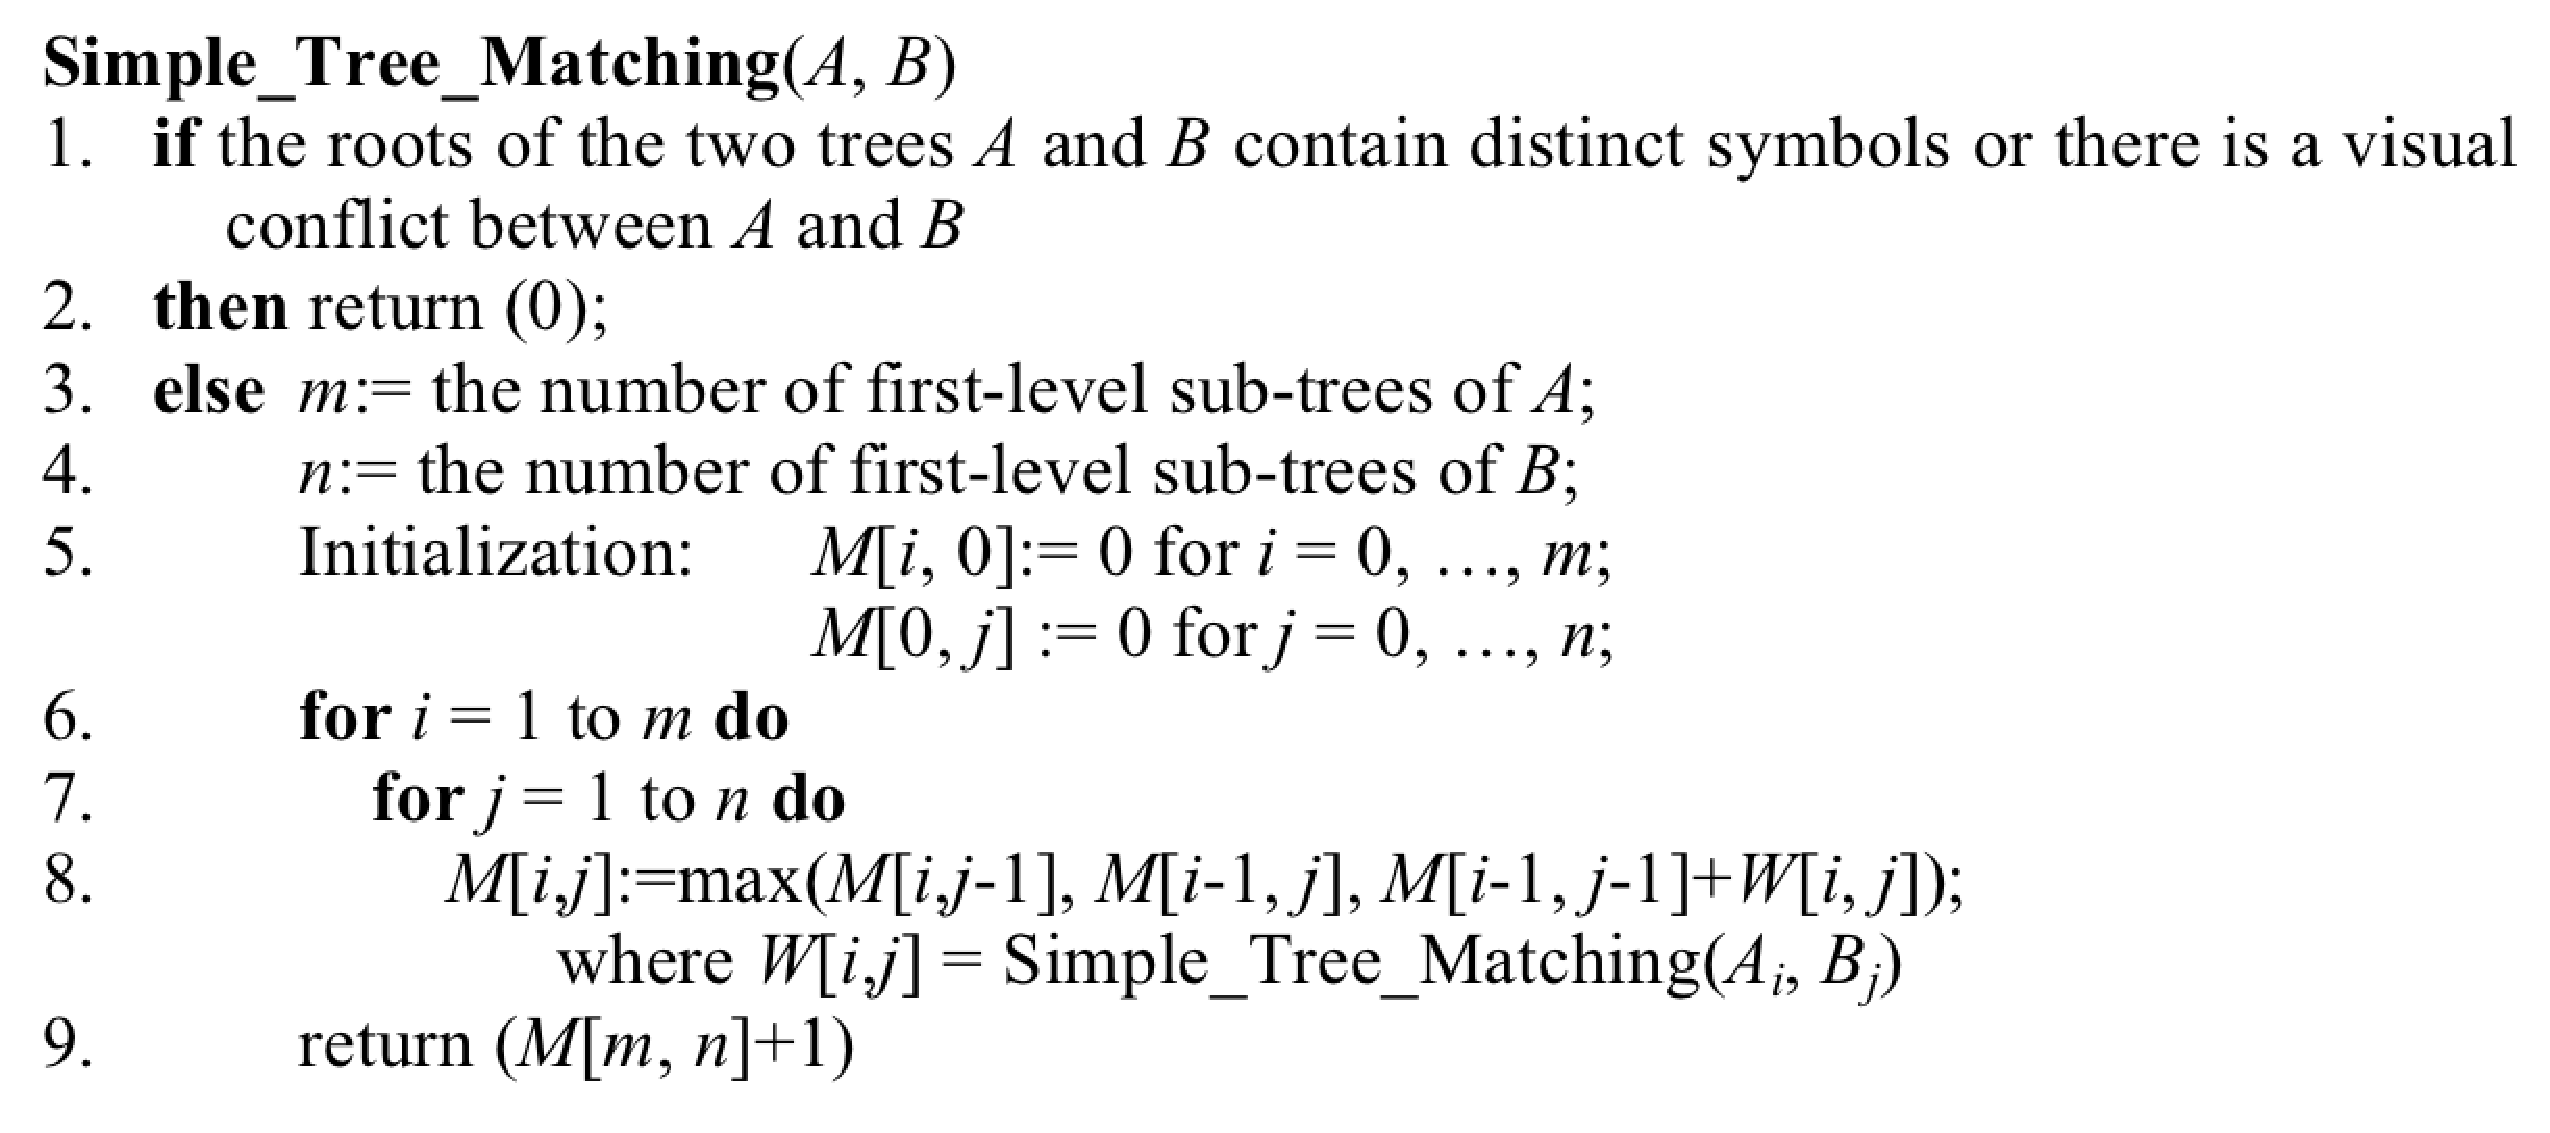
\includegraphics[width=\linewidth]{stm}

\end{frame}

% ------------------------------------------------------------

\begin{frame} \frametitle{An Example}

  \begin{block}{}
      \centering
      \includegraphics[width=.8\linewidth]{simple-tree-matching}
  \end{block}

  \vfill

  \centering

  \begin{tabular}{c|cccc}
      &   & B & C & D \\\hline
      & 0 & 0 & 0 & 0 \\
    B & 0 & \emph{\textbf{1}} & 1 & 1 \\
    C & 0 & 1 & 3 & 3 \\
    C & 0 & 1 & \emph{\textbf{4}} & 4 \\
  \end{tabular}\hfill
  \begin{tabular}{c|ccc}
      &   & E & F \\\hline
      & 0 & 0 & 0 \\
    E & 0 & \emph{\textbf{1}} & 1 \\
    G & 0 & 1 & 1 \\
  \end{tabular}\hfill
  \begin{tabular}{c|ccc}
      &   & E & F \\\hline
      & 0 & 0 & 0 \\
    E & 0 & \emph{\textbf{1}} & 1 \\
    F & 0 & 1 & \emph{\textbf{2}} \\
  \end{tabular}

  \alert{Matching = 5}\\[\baselineskip]
  
  %\small \uncover<2->{Question: How can this help in finding Web page
  %  templates?}

\end{frame}

% ------------------------------------------------------------

\section{An Example: RoadRunner}

\begin{frame}
    \frametitle{The RoadRunner Algorithm}
    
    \begin{itemize}
    \item RoadRunner is an algorithm for automatic wrapper generation
    \item Uses a \emph{nested-tuple representation} of the page schema
    \item Uses a \emph{RE-based model} of the extraction program
    \item It infers the schema and program from a given set of Web pages
    \end{itemize}

\end{frame}

% ------------------------------------------------------------

\newcommand{\pc}{\ensuremath{\#pcdata}}

% \begin{frame}
%     \frametitle{Union-Free Regular Expressions}
    
%     \begin{block}{Definition}
%         \begin{itemize}
%         \item Given an alphabet of symbols $\Sigma$ and a special token $\pc
%             \notin \Sigma$,
%         \item A UFRE over $\Sigma$ is a string over $\Sigma \cup \{\pc, +, ?,
%             (, )\}$ defined as follows:
%             \begin{itemize}
%             \item The empty string $\epsilon$ and all elements of $\Sigma \cup
%                 \{\pc\}$ are UFRE
%             \item If $A$ and $B$ are UFRE, then $AB$, $(A)+$ and $(A)?$ are
%                 regular expressions
%             \end{itemize}
%         \item Note: $(A)*$ stands for $((A)+)?$
%         \end{itemize}
%     \end{block}

%     \small Question: what is the difference from full regular expressions?

% \end{frame}

% ------------------------------------------------------------

\begin{frame}
    \frametitle{Union-Free Regular Expressions}
    
    \begin{itemize}
    \item<+-> RoadRunner explores the close correspondence between nested tuples
        and \emph{union-free regular expressions}
    \end{itemize}
      \begin{center}
          \begin{tabular}{c@{~~$\Rightarrow$~~}l}
              $\pc$ & value fields \\
              $+$ & (nested) lists \\
              $?$ & optional fields
          \end{tabular}
      \end{center}
    \begin{itemize}
    \item UFRE have limitations
        \begin{itemize}
        \item No disjunctions: it is not possible to code ``either A or B''
        \end{itemize}
    \item However, they are still a good approximation
        \begin{itemize}
        \item Capture most cases
        \item Simpler to process than full regular expressions
        \end{itemize}
    \end{itemize}
\end{frame}

% ------------------------------------------------------------

% \begin{frame}
%     \frametitle{Schema and program inference}
    
%     \begin{itemize}
%     \item Given a set of HTML strings $s_1, s_2, \dotsc, s_k$ that enconde a
%         set of items $i_1, i_2, \dotsc, i_k$ of type $\tau$, it is possible to
%         find the \emph{mininal UFRE} $\sigma$ whose language $L(\sigma)$
%         contains $s_1, s_2, \dotsc, s_k$.
%     \item The UFRE $\sigma$ can also be used as a wrapper to extract $i_1, i_2,
%         \dotsc, i_k$
%     \item Thus, solving the extraction problem consists in finding $\sigma$
%     \end{itemize}

% \end{frame}

% ------------------------------------------------------------

\begin{frame}
    \frametitle{The matching technique}
    
    \emph{ACME: Align, Collapse under Mismatch, and Extract}
    \begin{itemize}
    \item Two main items are processed:
        \begin{enumerate}
        \item The \emph{sample}: a list of tokens
        \item The \emph{wrapper}: a UFRE
        \end{enumerate}
    \item Given two Web pages $p_1$ and $p_2$:
        \begin{itemize}
        \item Use $p_1$ as the initial wrapper
        \item Use $p_2$ as the sample
        \item Parse the sample using the wrapper
        \item Generalize the wrapper by solving \textit{mismatches}
        \end{itemize}
    \end{itemize}

\end{frame}

% ------------------------------------------------------------

\begin{frame}
    \frametitle{Mismatches}
    
    Two types of mismatches:
    \begin{enumerate}
    \item \emph{String mismatches:} different strings occur at the same
        position of wrapper and sample
        \begin{itemize}
        \item Indicate the occurrence of field values
        \end{itemize}
    \item \emph{Tag mismatches:} different tags occur at the same position
        of wrapper and sample, or a string occurs where a tag should occur
        \begin{itemize}
        \item Indicate the occurrence of optional fields
        \item Or the occurrence of lists
        \end{itemize}
    \end{enumerate}

\end{frame}

% ------------------------------------------------------------

\begin{frame}
    \frametitle{Discovering fields}

    \begin{center}        
        % wrapper --- sample
        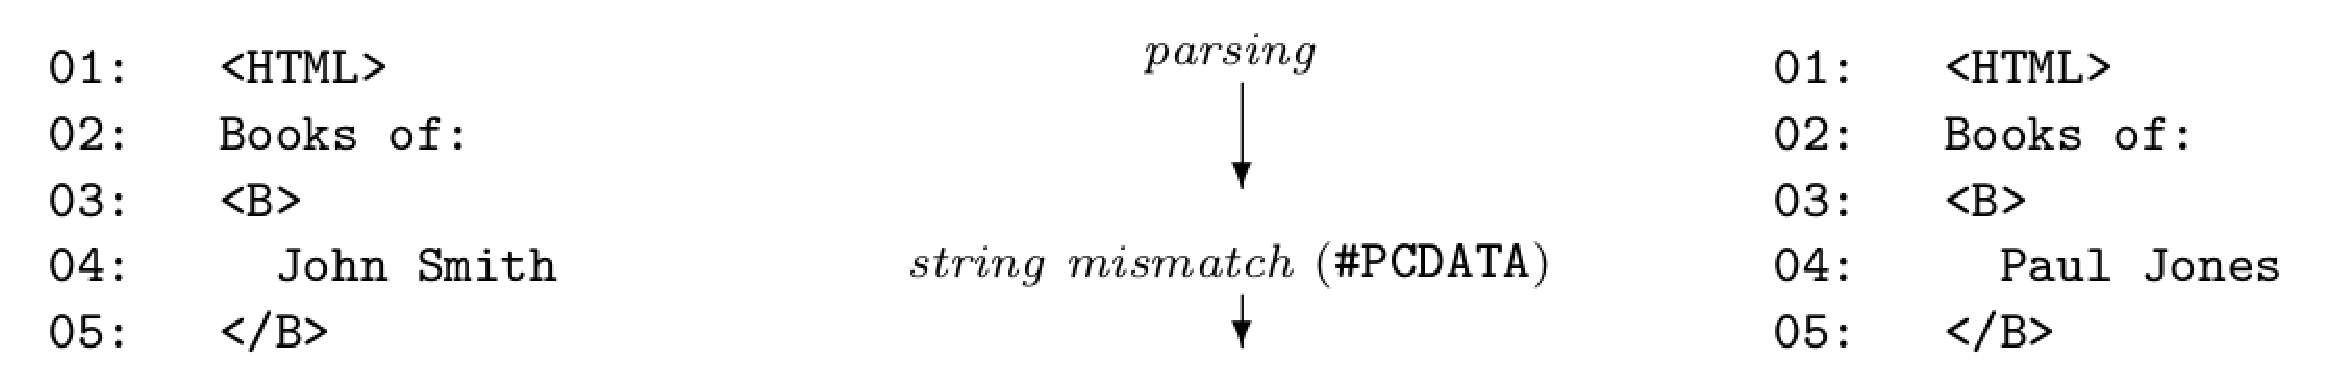
\includegraphics[width=\linewidth]{string-mismatch}
    \end{center}

    \emph{Wrapper generalization:}
    \begin{itemize}
    \item<2-> Replaced the mismatch with $\pc$
    \end{itemize}

\end{frame}

% ------------------------------------------------------------

\begin{frame}
    \frametitle{Discovering optional fields}
    
    \begin{center}        
        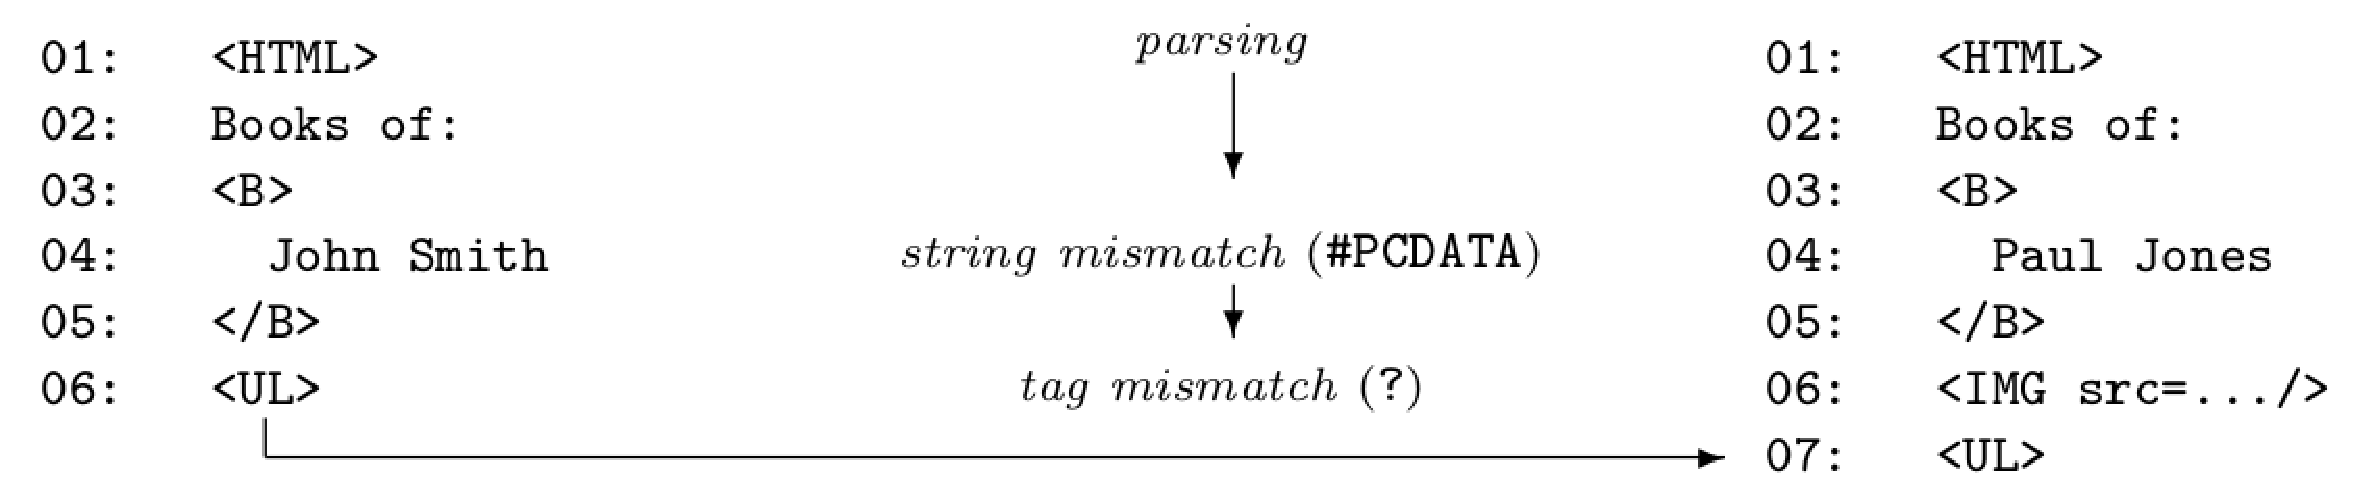
\includegraphics[width=\linewidth]{tag-mismatch}
    \end{center}

    \emph{Pattern location:}
    \begin{itemize}
    \item<2-> Pattern is in the wrapper (\texttt{<UL>}): locate \texttt{<IMG src=.../>} in the
        wrapper
    \item<2-> Pattern is in the sample (\texttt{<IMG>}): locate \texttt{<UL>} in
        the sample
    \end{itemize}

    \emph{Wrapper generalization:}
    \begin{itemize}
    \item<3-> Insert optional pattern in wrapper
        \begin{itemize}
        \item e.g. \texttt{(<IMG src=.../>)?}
        \end{itemize}
    \end{itemize}
    
\end{frame}

% ------------------------------------------------------------

\begin{frame}
    \frametitle{Discovering lists}
    
    \begin{center}        
        \includegraphics<+->[width=\linewidth]{list-mismatch}
    \end{center}

    Discover the \emph{square} location:
    \begin{enumerate}
    \item Find the \emph{terminal tag}
        \begin{itemize}
        \item<+-> We know that some squares have been matched
        \item<+-> Thus, if we go one step backwards, we find the fininshing tag
        \end{itemize}
    \item Find the \emph{initial tag}
        \begin{itemize}
        \item<+-> The mismatch indicates the end of the list on one side and
            the begining of the square on the other
            \begin{itemize}
            \item We don't know which side is which (is it \texttt{</UL>} or
                \texttt{</LI>}?)
            \end{itemize}
        \item<+-> Search the wrapper for \texttt{</UL>...</LI>}
        \item<+-> Search the sample for \texttt{<LI>...</LI>}
            % search from the point of the mismatch
        \end{itemize}
    \end{enumerate}
    
\end{frame}

% ------------------------------------------------------------

\begin{frame}
    \frametitle{Discovering lists (cont.)}
    
    \begin{center}        
        \includegraphics<+->[width=\linewidth]{list-mismatch}
    \end{center}

    \emph{Square matching} (to check if it is a true square)
    \begin{itemize}
    \item<+-> Search for matches backwards
        \begin{itemize}
        \item Match 25 and 19, match 24 and 18, ...
        \end{itemize}
    \item<+-> Stop when full square is matched
        \begin{itemize}
        \item I.e., when 20 and 14 match
        \end{itemize}
    \end{itemize}
    
\end{frame}

% ------------------------------------------------------------

\begin{frame}
    \frametitle{Discovering lists (cont.)}
    
    \begin{center}        
        \includegraphics<+->[width=\linewidth]{list-mismatch}
    \end{center}

    \emph{Wrapper generalization}
    \begin{itemize}
    \item<+-> Replace sequences of squares in the wrapper with the generalized
        expression
    \end{itemize}
    \begin{center}
        \only<.->{\texttt{(<LI><I>Title:</I>\pc</LI>)+}}
    \end{center}
    
\end{frame}

% ------------------------------------------------------------

\begin{frame}
    \frametitle{Final wrapper}
    
    \centering
    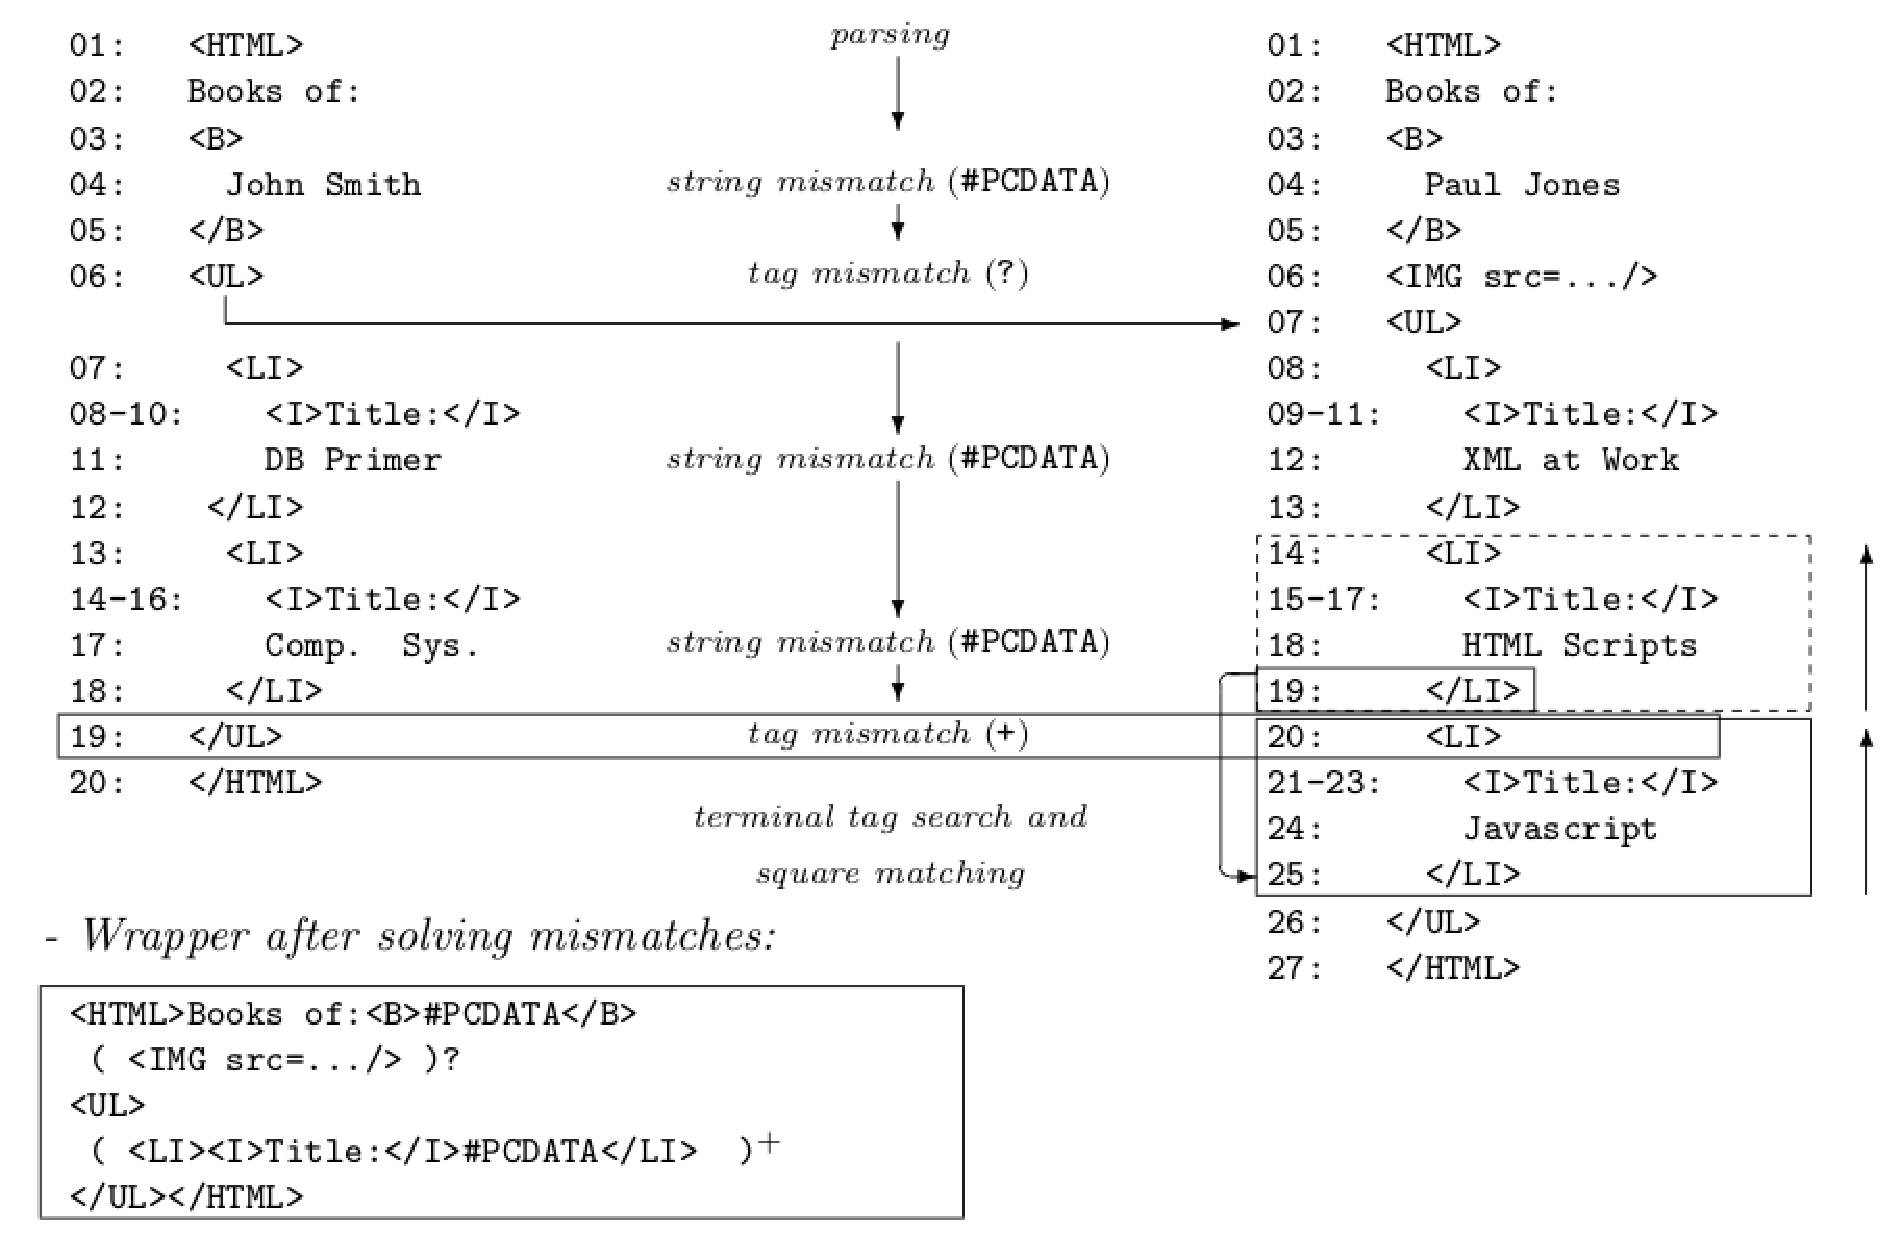
\includegraphics[width=\linewidth]{roadrunner-example}

    % \small\raggedleft Note: we must look for lists before optionals. Why?
    
\end{frame}

% ------------------------------------------------------------

\begin{frame}
    \frametitle{The need for recursion}
    
    \begin{itemize}
    \item Solving one mismatch may cause other mismatches to be found
        \begin{itemize}
        \item E.g., when matching squares on a list
        \end{itemize}
    \item These are called \emph{internal mismatches}
    \item They must be solved \emph{recursively}
    \end{itemize}

\end{frame}

% ------------------------------------------------------------

% \begin{frame}
%     \frametitle{The need for recursion (example)}
    
%     \centering
%     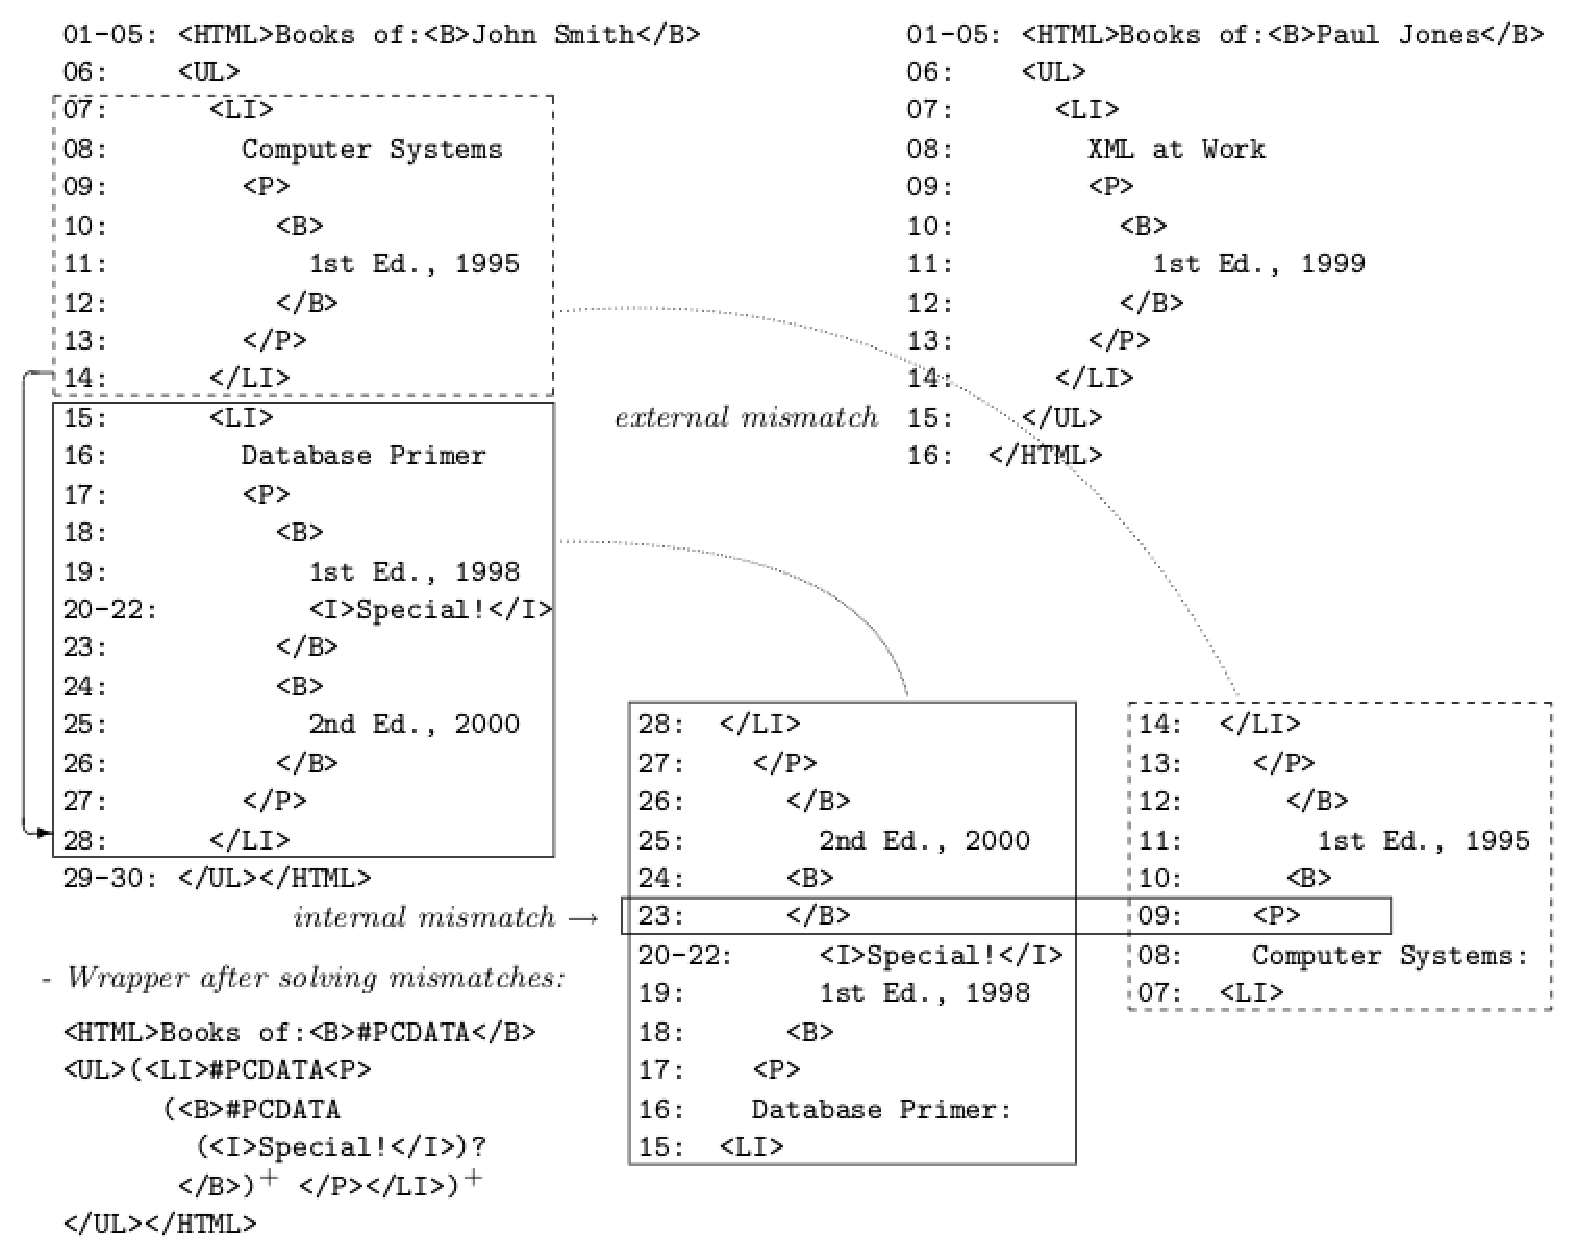
\includegraphics[width=\linewidth]{recursion}

% \end{frame}

% % ------------------------------------------------------------

% \begin{frame}
%     \frametitle{Backtracking}
    
%     \begin{itemize}
%     \item When matching, not all alternatives leed to the correct solution
%     \item Example:
%         \begin{itemize}
%         \item When looking for candidate squares, we may find many incorrect
%             initial and terminal tags
%         \end{itemize}
%     \item If a solution is not found, \emph{backtracking} must be performed
%     \end{itemize}

% \end{frame}

% % ------------------------------------------------------------

% \begin{frame}
%     \frametitle{Solving an AND-OR tree}
    
%     \begin{itemize}
%     \item Matching can be seen as solving an \emph{\href{http://en.wikipedia.org/wiki/And\%E2\%80\%93or_tree}{AND-OR tree}}
%     \end{itemize}

%     \begin{center}
%         \includegraphics[width=\linewidth]{and-or}
%     \end{center}

% \end{frame}

% % ------------------------------------------------------------

% \begin{frame}
%     \frametitle{Lowering the complexity}
    
%     \begin{itemize}
%     \item Matching is an exponential problem
%         \begin{itemize}
%         \item Worst case: exploring the full AND-OR tree
%         \end{itemize}
%     \item Can be optimized through \emph{pruning}
%     \end{itemize}

%     \begin{block}<+->{Pruning strategies:}
%         \begin{enumerate}
%         \item<+-> Limit the number of candidate optionals/squares
%             \begin{itemize}
%             \item The correct candidate is usually close to the mismatch
%             \end{itemize}
%         \item<+-> Do not backtrack if the chance of being wrong is very low
%             \begin{itemize}
%             \item E.g., if there was a match for a list (externally) , do not
%                 check if it was an optional
%             \end{itemize}
%         \item<+-> Ignore unlikely patterns
%             \begin{itemize}
%             \item E.g., optionals/iterators delimeted by optional patterns,
%                 such as \texttt{((<HR>)?<LI>\pc</LI>)+}
%             \end{itemize}

%         \end{enumerate}
%     \end{block}

% \end{frame}

% ------------------------------------------------------------

\section{Conclusion}

\begin{frame} \frametitle{Summary}

  Wrapper induction
  \begin{itemize}
  \item Advantages:
    \begin{itemize}
    \item Only the target data are extracted as the user can label only data
      items that he/she is interested in.
    \item Due to manual labeling, there is no integration issue for data
      extracted from multiple sites as the problem is solved by the user.
    \end{itemize}
  \item Disadvantages:
    \begin{itemize}
    \item It is not scalable to a large number of sites due to significant
      manual efforts. Even finding the pages to label is non-trivial.
    \item Wrapper maintenance (verification and repair) is very costly if the
      sites change frequently.
    \end{itemize}
  \end{itemize}

\end{frame}

% ------------------------------------------------------------

\begin{frame} \frametitle{Summary (cont.)}

  Automatic extraction
  \begin{itemize}
  \item Advantages:
    \begin{itemize}
    \item It is scalable to a huge number of sites due to the automatic
      process.
    \item There is little maintenance cost.
    \end{itemize}
  \item Disadvantages:
    \begin{itemize}
    \item It may extract a large amount of unwanted data because the system
      does not know what is interesting to the user. Domain heuristics or
      manual filtering may be needed to remove unwanted data.
    \item Extracted data from multiple sites need integration, i.e., their
      schemas need to be matched.
    \end{itemize}
  \end{itemize}

\end{frame}

% ------------------------------------------------------------

\begin{frame} \frametitle{Summary (cont.)}

  Conclusions
  \begin{itemize}
  \item In terms of extraction accuracy, it is reasonable to assume that
    wrapper induction is more accurate than automatic extraction. However,
    there is no reported comparison.
  \item Applications
    \begin{itemize}
    \item Wrapper induction should be used in applications in which the number
      of sites to be extracted and the number of templates in these sites are
      not large.
    \item Automatic extraction is more suitable for large scale extraction
      tasks which do not require accurate labeling or integration.
    \end{itemize}
  \end{itemize}

  \begin{center}
      \emph{Still an active research area!}
  \end{center}

\end{frame}

% ------------------------------------------------------------
% ------------------------------------------------------------
% ------------------------------------------------------------
% ------------------------------------------------------------

\begin{frame}
    \frametitle{References}
    
    \begin{itemize}
    \item Ion Muslea, Steve Minton, Craig Knoblock. \emph{Stalker: Learning
          extraction rules for semistructured, web-based information
          sources}. Proceedings of AAAI-98 Workshop on AI and Information
        Integration.
    \item Bing Liu and Yanhong Zhai. \emph{NET --- A System for Extracting Web
          Data from Flat and Nested Data Records}. Proceedings of 6th
        International Conference on Web Information Systems Engineering
        (WISE-05).
    \item Valter Crescenzi, Giansalvatore Mecca, Paolo
        Merialdo. \emph{RoadRunner: Towards Automatic Data Extraction from
          Large Web Sites}. Proceedings of the 27th VLDB Conference, Roma,
        Italy, 2001.
    \end{itemize}

\end{frame}

% ------------------------------------------------------------

\finalframe{\Large{Questions?}}

% ------------------------------------------------------------
% ------------------------------------------------------------
% ------------------------------------------------------------
% ------------------------------------------------------------

\end{document}

%%% Local Variables: 
%%% mode: latex
%%% TeX-master: t
%%% End: 
